% !TEX root = metrics_pro_en.tex
% !TEX root = metrics_pro.tex

\maketitle

% сюда поставим прикольную картинку

\newpage

\tableofcontents{}


% \maketitle % ставим сюда название, автора и время создания


\newpage
\section{\trru{МНК — это\ldots} \tren{OLS is\dots}}

\begin{translationru}
\begin{leftbar}
Истинная модель. Например, $y_i = \beta_1 + \beta_2 x_i + \beta_3 z_i + u_i$.

Формула для прогнозов. Например, $\hy_i = \hb_1 + \hb_2 x_i + \hb_3 z_i$.

Метод наименьших квадратов, $\sum (y_i - \hy_i)^2 \to \min$.  
\end{leftbar}  
\end{translationru}

\begin{translationen}
\begin{leftbar}
True model. For example, $y_i = \beta_1 + \beta_2 x_i + \beta_3 z_i + u_i$.

Forecasting formula. For example, $\hy_i = \hb_1 + \hb_2 x_i + \hb_3 z_i$.

Ordinary least squares, $\sum (y_i - \hy_i)^2 \to \min$.  
\end{leftbar}  
\end{translationen}
  


\begin{problem}
\begin{translationru}
Каждый день Маша ест конфеты и решает задачи по эконометрике. Пусть $x_i$ — количество решённых задач, а $y_i$ — количество съеденных конфет.

\begin{tabular}{cc}
\toprule
$x_i$ & $y_i$ \\
\midrule
1 & 1 \\
2 & 2 \\
2 & 4 \\
\bottomrule
\end{tabular}

Рассмотрим модель $y_i = \beta x_i + u_i$.

\begin{enumerate}
\item Найдите МНК-оценку $\hb$ для имеющихся трёх наблюдений.
\item Нарисуйте исходные точки и полученную прямую регрессии.
\item Выведите формулу для $\hb$ в общем виде для $n$ наблюдений.
\end{enumerate}

Рассмотрим модель $y_i = \beta_1 + \beta_2 x_i + u_i$.
\begin{enumerate}[resume]
\item Найдите МНК-оценки $\hb_1$ и $\hb_2$ для имеющихся трёх наблюдений.
\item Нарисуйте исходные точки и полученную прямую регрессии.
\item Выведите формулу для $\hb_2$ в общем виде для $n$ наблюдений.
\end{enumerate}
\end{translationru}

\begin{translationen}
Everyday Maria eats candies and solves econometrics problems.
Let $x_i$ be the number of problems solved and $y_i$ be the number of candies eaten.

\begin{tabular}{cc}
\toprule
$x_i$ & $y_i$ \\
\midrule
1 & 1 \\
2 & 2 \\
2 & 4 \\
\bottomrule
\end{tabular}

Consider the model $y_i = \beta x_i + u_i$.

\begin{enumerate}
\item Find the OLS estimate $\hb$ for the toy dataset.
\item Draw original points and estimated regression line on a graph.
\item Derive the general formula for $\hb$ in the case of $n$ observations.
\end{enumerate}

Now consider the model $y_i = \beta_1 + \beta_2 x_i + u_i$.
\begin{enumerate}[resume]
\item Find the OLS estimates $\hb_1$ and $\hb_2$ for the toy dataset.
\item Draw original points and estimated regression line on a graph.
\item Derive the general formula for $\hb$ in the case of $n$ observations.
\end{enumerate}
\end{translationen}

\begin{sol}
\begin{enumerate}
\item $\hb = 13/9$;
\item 
\item $\hb = \frac{\sum_{i=1}^n x_i y_i}{\sum_{i=1}^n x_i^2}$;
\item $\hb_1 = -1$, $\hb_2 = 2$;
\item 
\item $\hb_2 = \frac{\sum_{i=1}^n (x_i - \bar x)(y_i - \bar y)}{\sum_{i=1}^n (x_i - \bar x)^2}$.
\end{enumerate}
\end{sol}
\end{problem}


\begin{problem}
\trru{Докажите формулы или приведите контр-пример:}
\tren{Prove the following formulas or provide a counter-example:}
\begin{enumerate}
\item $\sum_{i}(x_i - \bar x)^2 = \sum_i (x_i - \bar x) x_i$;
\item $\sum_{i}(x_i - \bar x)(y_i - \bar y) = \sum_i (x_i - \bar x) y_i$;
\item $\sum_{ij}(x_i - x_j)^2 = 2 n \sum_i(x_i - \bar x)^2$;
\item $\sum_{ij}(x_i - x_j)(y_i - y_j) = 2 \sum_i(x_i - \bar x)(y_i - \bar y)$;
\item $\sum_{i}(x_i - \bar x)(y_i - \bar y) = \sum_i x_i  y_i$;
\end{enumerate}

\begin{sol}
\begin{translationru}
\begin{enumerate}
\item верная формула;
\item верная формула;
\item верная формула;
\item неверная формула, верная имеет вид $\sum_{ij}(x_i - x_j)(y_i - y_j) = 2 n\sum_i(x_i - \bar x)(y_i - \bar y)$;
\item неверная формула, верная имеет вид $\sum_{i}(x_i - \bar x)(y_i - \bar y) = \sum_i x_i  y_i - n \bar x \bar y$.
\end{enumerate}            
\end{translationru}

\begin{translationen}
\begin{enumerate}
\item correct;
\item correct;
\item correct;
\item wrong, correct formula should be $\sum_{ij}(x_i - x_j)(y_i - y_j) = 2 n\sum_i(x_i - \bar x)(y_i - \bar y)$;
\item wrong, correct formula should be $\sum_{i}(x_i - \bar x)(y_i - \bar y) = \sum_i x_i  y_i - n \bar x \bar y$.
\end{enumerate}            
\end{translationen}
    
\end{sol}
\end{problem}
  


\begin{problem}
\trru{Упростите выражения:}
\tren{Simplify the following expressions:}
\begin{enumerate}
\item $n\bar x - \sum x_i$;
\item $\sum (x_i - \bar x)\bar x$;
\item $\sum (x_i - \bar x)\bar z$;
\item $\sum (x_i - \bar x)^2 + n \bar{x}^2$.
\end{enumerate}

\begin{sol}
\begin{enumerate}
\item $0$
\item $0$
\item $0$
\item $\sum x_i^2$
\end{enumerate}
\end{sol}
\end{problem}


\begin{problem}
\trru{При помощи метода наименьших квадратов найдите оценку неизвестного параметра $\theta$ в следующих моделях:}
\tren{Using OLS find the estimator $\theta$ in the following models:}

\begin{enumerate}
\item $y_i = \theta + \theta x_i + \varepsilon_i$;
\item $y_i = 1 + \theta x_i + u_i$;
\item $y_i = \theta / x_i + u_i$;
\item $y_i = \theta x_i + (1-\theta)z_i+u_i$.
\end{enumerate}

\begin{sol}
\begin{enumerate}
\item $\htheta = \frac{\sum y_i (1 + x_i)}{\sum (1 + x_i)^2}$
\item $\htheta = \frac{\sum (y_i - 1) x_i}{\sum x_i^2}$
\item $\htheta = \frac{\sum (y_i / x_i)}{\sum (1 / x_i^2)}$
\item $\htheta = \sum \left((y_i - z_i)(x_i - z_i) \right) / \sum \left(x_i - z_i\right)^2$
\end{enumerate}
\end{sol}
\end{problem}

\begin{problem}
\begin{translationru}
    Найдите МНК-оценки параметров $\alpha$ и $\beta$ в модели $y_i = \alpha + \beta y_i + u_i$.    
\end{translationru}
\begin{translationen}
    Find the OLS estimators $\alpha$ and $\beta$ for the model $y_i = \alpha + \beta y_i + u_i$.    
\end{translationen}

\begin{sol}
$\hat{\alpha} = 0,  \hb = 1$
\end{sol}
\end{problem}


\begin{problem}
Рассмотрите модели $y_i = \alpha + \beta (y_i + z_i) + u_i$, $z_i = \gamma + \delta(y_i+z_i) + u_i$.
\begin{enumerate}
\item Как связаны между собой $\hat{\alpha}$ и $\hat{\gamma}$?
\item Как связаны между собой $\hb$ и $\hat{\delta}$?
\end{enumerate}


\begin{sol} % 1.5.
Рассмотрим регрессию суммы $(y_i + z_i)$ на саму себя. Естественно, в ней
\[
\widehat{y_i + z_i} = 0 + 1 \cdot (y_i + z_i).
\]

Отсюда получаем, что $\hat{\alpha} + \hat{\gamma} = 0$ и $\hb + \hat{\delta} = 1$.
\end{sol}
\end{problem}




\begin{problem}
Как связаны МНК-оценки параметров $\alpha, \beta$ и $\gamma, \delta$ в моделях $y_i = \alpha + \beta x_i + u_i$ и $z_i = \gamma + \delta x_i + \upsilon_i$, если $z_i = 2 y_i$?


\begin{sol}

Исходя из условия, нужно оценить методом МНК коэффициенты двух следующих моделей:
\[y_i = \alpha + \beta x_i + u_i \]
\[y_i = \frac{\gamma}{2} + \frac{\delta}{2} x_i + \frac{1}{2} v_i \]

Заметим, что на минимизацию суммы квадратов остатков коэффициент \(1/2\) не влияет, следовательно:
\[\hat{\gamma} = 2\hat{\alpha}, \ \hat{\delta} = 2 \hb  \]

\end{sol}
\end{problem}


\begin{problem}
Для модели $y_i = \beta_1 x_i + \beta_2 z_i + u_i$ решите условную задачу о наименьших квадратах:
\[
Q(\beta_1, \beta_2) := \sum_{i=1}^n (y_i - \hb_1 x_i - \hb_2 z_i)^2 \to \underset{\hb_1 + \hb_2 = 1}{\min}.
\]


\begin{sol}
Выпишем задачу:
\[
\begin{cases}
RSS = \sum_{i=1}^{n}(y_i - \hb_1x_i - \hb_2z_i)^2 \to \min_{\hb_1, \hb_2}\\
\hb_1 + \hb_2 = 1
\end{cases}
\]

Можем превратить ее в задачу минимизации функции одного аргумента:
\[
RSS =  \sum_{i=1}^{n}(y_i - x_i - \hb_2(z_i-x_i))^2 \to \min_{\hb_2}
\]

Выпишем условия первого порядка:
\[
\frac{\partial RSS}{\partial \hb_2} = \sum_{i=1}^{n}2(y_i-x_i-\hb_2(z_i-x_i))(x_i-z_i)=0
\]

Отсюда:
\[
\sum_{i=1}^{n}(y_i-x_i)(x_i-z_i) + \hb_2\sum_{i=1}^{n}(z_i-x_i)^2 = 0 \Rightarrow \hb_2 = \frac{\sum_{i=1}^n (y_i-x_i)(z_i-x_i)}{\sum_{i=1}^n (z_i-x_i)^2}
\]

А $\hb_1$ найдется из соотношения $\hb_1+\hb_2 = 1$.

\end{sol}
\end{problem}

\begin{problem}
Перед нами два золотых слитка и весы, производящие взвешивания с ошибками. Взвесив первый слиток, мы получили результат $300$ грамм, взвесив второй слиток — $200$ грамм, взвесив оба слитка — $400$ грамм. Оцените вес каждого слитка методом наименьших квадратов.

\begin{sol}
Обозначив вес первого слитка за \(\beta_1\), вес второго слитка за \(\beta_2\), а показания весов за \(y_i\), получим, что
\[y_1 = \beta_1 + u_1, \ y_2 = \beta_2 + u_2, \ y_3 = \beta_1 + \beta_2 + u_3\]

Тогда
\[(300 - \beta_1)^2 + (200 - \beta_2)^2 + (400 - \beta_1 - \beta_2)^2 \to \min _{\beta_1,\  \beta_2} \]
\[\hb_1 = \frac{800}{3}, \ \hb_2 = \frac{500}{3} \]
\end{sol}
\end{problem}


\begin{problem}
Аня и Настя утверждают, что лектор опоздал на 10 минут. 
Таня считает, что лектор опоздал на 3 минуты. 
С помощью МНК оцените, на сколько опоздал лектор.

\begin{sol}
Можем воспользоваться готовой формулой для регрессии на константу:
\[
\hb = \bar{y} = \frac{10+10+3}{3} = \frac{23}{3}
\]

(можно решить задачу $2(10-\beta)^2 + (3-\beta)^2\to \min$)

\end{sol}
\end{problem}

\begin{problem}
Есть двести наблюдений. Вовочка оценил модель $\hy_i=\hb_1+\hb_2 x_i$ по первой сотне наблюдений.
Петечка оценил модель $\hy_i=\hat{\gamma}_1+\hat{\gamma}_2 x_i$ по второй сотне наблюдений.
Машенька оценила модель $\hy_i=\hat{\phi}_1+\hat{\phi}_2 x_i$ по всем наблюдениям.
\begin{enumerate}
\item Возможно ли, что $\hb_2>0$, $\hat{\gamma}_2>0$, но $\hat{\phi}_2<0$?
\item Возможно ли, что $\hb_1>0$, $\hat{\gamma}_1>0$, но $\hat{\phi}_1<0$?
\item Возможно ли одновременное выполнение всех упомянутых условий?
\item Возможно ли одновременное выполнение всех упомянутых условий,
если в каждой сотне наблюдений $\sum x_i > 0$?
\end{enumerate}

\begin{sol}
\begin{enumerate}
\item Да.
\item Да.
\item Да.
\item Нет. Из условия первого порядка для первой выборки следует,
что $\sum_A y_i = \hb_1 + \hb_2 \sum x_i$. Значит $\sum_A y_i > 0$. Аналогично, $\sum_B y_i >0$,
но $\sum y_i <0$.
\end{enumerate}
\end{sol}
\end{problem}


\begin{problem}

Эконометрист Вовочка собрал интересный набор данных по студентам третьего курса:
\begin{itemize}
\item переменная $y_i$ — количество пирожков, съеденных $i$-ым студентом за прошлый год;
\item переменная $f_i$, которая равна 1, если $i$-ый человек в выборке — женщина, и 0, если мужчина.
\item переменная\footnote{Это нетолерантная задача и здесь либо $f$ равно 1, либо $m$} $m_i$, которая равна 1, если $i$-ый человек в выборке — мужчина, и 0, если женщина.
\end{itemize}

Вовочка оценил 4 регрессии:
\begin{enumerate}
\item[A:] $y$ на константу и $f$, $\hy_i = \hat \alpha_1 + \hat \alpha_2 f_i$;
\item[B:] $y$ на константу и $m$, $\hy_i = \hb_1 + \hb_2 m_i$;
\item[C:] $y$ на $f$ и $m$ без константы, $\hy_i = \hat \gamma_1 f_i + \hat \gamma_2 m_i$;
\item[D:] $y$ на константу, $f$ и $m$, $\hy_i = \hat \delta_1 + \hat \delta_2 f_i + \hat \delta_3 m_i$;
\end{enumerate}

\begin{enumerate}
\item Какой смысл будут иметь оцениваемые коэффициенты?
\item Как связаны между собой оценки коэффициентов этих регрессий?
\end{enumerate}


\begin{sol}
\end{sol}
\end{problem}


\begin{problem}
Эконометрист Вовочка оценил методом наименьших квадратов модель 1, $y_i=\beta_1+\beta_2 x_i+\beta_3 z_i+u_i$,
а затем модель 2, $y_i=\beta_1+\beta_2 x_i+\beta_3 z_i+\beta_4 w_i+u$.
Сравните полученные $ESS$, $RSS$, $TSS$ и $R^2$.

\begin{sol}
Поскольку значения $y$ остались теми же, $TSS_1 = TSS_2$.

Добавление ещё одного регрессора не уменьшит точность оценки, то есть
$RSS_2 \leq RSS_1$, $ESS_2 \geq ESS_1$.

Тогда и коэффициент детерминации $R^2 = ESS / TSS$ не уменьшится, то есть
$R^2_2 \geq R^2_1$.
\end{sol}
\end{problem}

\begin{problem}
Что происходит с $TSS$, $RSS$, $ESS$, $R^2$ при добавлении нового наблюдения? Если величина может изменяться только в одну сторону, то докажите это. Если возможны и рост, и падение, то приведите пример.


\begin{sol}
Пусть \(\bar{y}\) — средний \(y\) до добавления нового наблюдения, \(\bar{y}'\) — после добавления нового наблюдения. Будем считать, что изначально было \(n\) наблюдений. Заметим, что
\[\bar{y}' = \frac{(y_1 + \ldots + y_n) + y_{n+1}}{n + 1} = \frac{n \bar{y} + y_{n + 1}}{n + 1} = \frac{n}{n+ 1}\bar{y} + \frac{1}{n+1}y_{n+1}\]

Покажем, что \(TSS\) может только увеличится при добавлении нового наблюдения (остается неизменным при \(y_{n+1} = \bar{y}\)):
\[TSS'= \sum_{i = 1}^{n + 1} (y_i - \bar{y}')^2 = \sum_{i = 1}^{n} (y_i - \bar{y} + \bar{y} - \bar{y}')^2 + (y_{n + 1} - \bar{y}')^2 = \]
\[=\sum_{i = 1}^{n} (y_i - \bar{y})^2 + n(\bar{y} - \bar{y}')^2 + (y_{n + 1} - \bar{y}')^2  = TSS + \frac{n}{n+1} (y_{n+1} - \bar{y})^2\]

Следовательно, \(TSS' \geq TSS\).

Также сумма \(RSS\) может только вырасти или остаться постоянной при добавлении нового наблюдения. Действительно, новое $(n+1)$-ое слагаемое в сумме неотрицательно. А сумма $n$ слагаемых минимальна при старых коэффициентах, а не при новых.

\(ESS\) и \(R^2\) могут меняться в обе стороны. Например, рассмотрим ситуацию, где точки лежат симметрично относительно некоторой горизонтальной прямой. При этом $ESS=0$. Добавим наблюдение — $ESS$ вырастет, удалим наблюдение — $ESS$ вырастет.
\end{sol}
\end{problem}



\begin{problem}
Эконометресса Аглая подглядела, что у эконометрессы Жозефины получился $R^2$ равный $0.99$ по 300 наблюдениям. От чёрной зависти Аглая не может ни есть, ни спать.

\begin{enumerate}
\item Аглая добавила в набор данных Жозефины ещё 300 наблюдений с такими же регрессорами, но противоположными по знаку игреками, чем были у Жозефины. Как изменится $R^2$?
\item Жозефина заметила, что Аглая добавила 300 наблюдений и вычеркнула их, 
вернув набор данных в исходное состояние. Хитрая Аглая решила тогда добавить всего одно наблюдение так, чтобы $R^2$ упал до нуля. 
Удастся ли ей это сделать?
\end{enumerate}


\begin{sol}
\begin{enumerate}
\item $R^2$ упал до нуля.
\item Да, можно. Если добавить точку далеко слева внизу от исходного набора данных, то наклон линии регрессии будет положительный. Если далеко справа внизу, то отрицательный. Будем двигать точку так, чтобы поймать нулевой наклон прямой. Получим $ESS=0$.
\end{enumerate}
\end{sol}
\end{problem}


\begin{problem}
\trru{На работе Феофан построил парную регрессию по трём наблюдениям и посчитал прогнозы $\hat{y}_i$. Придя домой он отчасти вспомнил результаты:

\begin{tabular}{rr}
\toprule
$y_i$ & $\hy_i$ \\
\midrule
$0$ & $1$ \\
$6$ & ? \\
$6$ & ? \\
\bottomrule
\end{tabular}

Поднапрягшись, Феофан вспомнил, что третий прогноз был больше второго.
Помогите Феофану восстановить пропущенные значения.}
\tren{Foma estimated simple regression model using three observations and calculated the forecasts $\hat{y}_i$. 
Unfortunately he remembers only this table:

\begin{tabular}{rr}
\toprule
$y_i$ & $\hy_i$ \\
\midrule
$0$ & $1$ \\
$6$ & ? \\
$6$ & ? \\
\bottomrule
\end{tabular}

He recalls that $\hat y_3 > \hat y_2$. 

Help Foma to reconstruct the missing entries in the table. 
}


\begin{sol}
На две неизвестных $a$ и $b$ нужно два уравнения. Эти два уравнения — ортогональность вектора остатков плоскости регрессоров. А именно:

\[
\begin{cases}
\sum_i (y_i - \hy_i) = 0 \\
\sum_i (y_i - \hy_i) \hy_i = 0 \\
\end{cases}
\]

В нашем случае

\[
\begin{cases}
-1 +(6-a) + (6-b) = 0 \\
-1 + (6 - a)a + (6-b)b = 0 \\
\end{cases}
\]

Решаем квадратное уравнение и получаем два решения: $a=4$ и $a=7$. Итого: $a=4$, $b=7$.
\end{sol}
\end{problem}


\begin{problem}
Вся выборка поделена на две части. Возможны ли такие ситуации:
\begin{enumerate}
    \item Выборочная корреляция между $y$ и $x$ примерно равна нулю в каждой части,
    а по всей выборке примерно равна единице;
    \item Выборочная корреляция между $y$ и $x$ примерно равна единице в каждой части,
    а по всей выборке примерно равна нулю?
\end{enumerate}

\begin{sol}
Обе ситуации возможны.
\end{sol}
\end{problem}


\begin{problem}
Бесстрашный исследователь Ипполит оценил парную регрессию. При этом оказалось,
каждый $x_i >0$ и обе оценки коэффициентов $\hb_1$ и $\hb_2$ также положительны.

\begin{enumerate}
  \item Возможно ли, что среди $\hat y_i$ есть отрицательные? Среди $y_i$ есть отрицательные?
  \item Возможно ли, что сумма $\sum \hat y_i$ отрицательна? Сумма $\sum y_i$ отрицательна?
  \item Как изменятся ответы, если известно, что $\sum x_i >0$?
\end{enumerate}

\begin{sol}
  \begin{enumerate}
    \item нет, да
    \item нет, нет
    \item да, да, нет, нет
  \end{enumerate}
\end{sol}
\end{problem}



\begin{problem}
\trru{Предложите способ подсчёта корреляции}
\tren{Propose a way to define a correlation}
\begin{enumerate}
  \item \trru{между бинарной переменной и факторной переменной;}
  \tren{between binary and factor variables;}
  \item \trru{между количественной переменной и факторной переменной.}
  \tren{between quantitative and factor variables.}
\end{enumerate}
  \begin{sol}
    \trru{Заменяем факторную переменную на набор бинарных предикторов. 
    С помощью этих предикторов прогнозируем бинарную или количественную переменную.
    Считаем $R^2$. Извлекаем корень.}
    \tren{Replace factor variable with indicators for every its value.
    Using this predictors obtain forecasts of binary or quantitative variable.
    Calculate $R^2$ and take the square root. }

  \end{sol}
\end{problem}
  



\begin{problem}
  Начинающий художник Франческо нарисовал облако из 1000 точек в осях $(x, y)$.
  Разные наблюдения независимы, для каждой пары точек $\Corr(x_i, y_i) = 0.5$.
  По отдельности величины $x_i$ и $y_i$ имеют стандартное нормальное распределение. 

  \begin{enumerate}
    \item Правда ли, что облако точек примерно симметрично относительно оси $x=y$?
    \item Воспроизведите примерно шедевр начинающего мастера. 
    \item Добавьте к облаку точек линии парных регрессий $y$ от $x$ и $x$ от $y$. 
  \end{enumerate}


\begin{sol}
  График примерно симметричен относительно $x=y$. 
  Линии регрессий примерно равны $\hat y_i \approx 0.5 x_i$ и $\hat x_i \approx 0.5 y_i$, 
  что при выражении в обычных координатах даёт $y_i\approx 2 \hat x_i$. 

  % \begin{minted}{r}
  \begin{lstlisting}[language=r]
    library(mvtnorm)
    library(tidyverse)
    
    V = matrix(c(1, 0.5, 0.5, 1), nrow = 2)
    xy = rmvnorm(n = 10^4, mean = c(0, 0), sigma = V)
    colnames(xy) = c('x', 'y')
    xy_df = as_tibble(xy)
    
    mod_yx = lm(data = xy_df, y ~ x)
    
    mod_xy = lm(data = xy_df, x ~ y)
    xy_slope = 1 / coef(mod_xy)[2]
    xy_int = - coef(mod_xy)[1] / coef(mod_xy)[2]
    
    qplot(data = xy_df, x = x, y = y) +
      geom_abline(slope = coef(mod_yx)[2], intercept = coef(mod_yx)[1], color = 'blue') +
      geom_abline(slope = 1, intercept = 0, color = 'red') +
      geom_abline(slope = xy_slope, intercept = xy_int, color = 'blue')
\end{lstlisting}
% \end{minted}



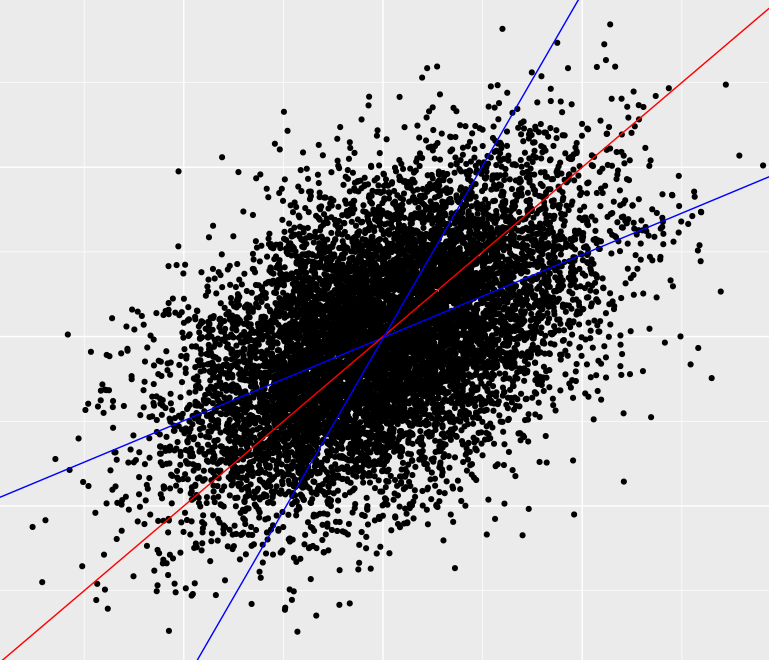
\includegraphics[scale=0.5]{figure/correlation_05.png}

\end{sol}
\end{problem}
  


\begin{problem}
Подающий надежды молодой художник Франческо увлекся минимализмом. 
Он нарисовал три точки на плоскости $(x, y)$ симметрично линии $x=y$ так, что
выборочные средние $\bar x = \bar y = 0$, выборочные дисперсии равны $1$.
А выборочная корреляция равна $0.5$.
\begin{enumerate}
\item Воспроизведите рисунок начинающего маэстро.
\item Добавьте на рисунок линии парных регрессий $y$ от $x$ и $x$ от $y$. 
\end{enumerate}
\begin{sol}
\end{sol}
\end{problem}



\begin{problem}
Усердный муравей Виталий вместо того, чтобы построить одну регрессию по $n$ точкам,
построил все возможные парные регрессии для каждой пары точек $(i, j)$.
При этом Виталий получил множество оценок коэффициентов $\hb_{1ij}$ и $\hb_{2ij}$.

Сами наблюдения не сохранились, однако для каждой пары точек помимо двух оценок также сохранился квадрат расстояния между ними по горизонтали
$q_{ij} = (x_i - x_j)^2$.

\begin{enumerate}
  \item Помогите Виталию восстановить классическую мнк-оценку $\hb_2$.
  \item Помогите Виталию восстановить классическую мнк-оценку $\hb_1$.
\end{enumerate}
\begin{sol}
  \begin{enumerate}
    \item $\hb_2 = \sum_{ij} w_{ij} \hb_{2ij}$, где веса считаются по формуле $w_{ij} = q_{ij} / \sum_{ij} q_{ij}$.
    \item $\hb_1 = \sum_{ij} w_{ij} \hb_{1ij}$.
  \end{enumerate}  
\end{sol}
\end{problem}
  



\section{\trru{Дифференциал — просто няшка!}
\tren{Fun with differential}}


\begin{leftbar}
\begin{itemize}
\item $d(A + B) = dA + dB$;
\item \trru{Если $A$ — матрица констант, то $dA = 0$;}
\tren{If $A$ is a constant matrix, then $dA = 0$;}
\item $d(AB) = dA \cdot B + A \cdot dB$;
\trru{Если $A$ — матрица констант, то $d(AB) = A \cdot dB$ и $d(BA) = dB \cdot A$;}
\tren{If $A$ is a constant matrix, then $d(AB) = A \cdot dB$ and $d(BA) = dB \cdot A$;}
\end{itemize}

\trru{Штрих у матрицы традиционно обозначает не производную, а транспонирование, $A'=A^T$.}
\tren{Transpose of a matrix is often denoted by prime, $A' = A^T$.}
\end{leftbar}

\begin{problem}
    Вспомним дифференциал :)
    \begin{enumerate}
        \item Известно, что $f(x) = x^2 + 3x$. Найдите $f'(x)$ и $df$. Чему равен $df$ в точке $x=5$ при $dx=0.1$?
        \item Известно, что $f(x_1, x_2)=x_1^2 + 3x_1x_2^3$. Найдите $df$. Чему равен $df$ в точке $x_1=-2$, $x_2=1$ при $dx_1=0.1$ и $dx_2=-0.1$?
        \item Известно, что $F=\begin{pmatrix}
                5 & 6x_1 \\
                x_1x_2 & x_1^2x_2 \\
            \end{pmatrix}$. Найдите $dF$.
        \item Известно, что $F=\begin{pmatrix}
                7 & 8 & 9 \\
                2 & -1 & -2 \\
            \end{pmatrix}$. Найдите $dF$.
        \item Матрица $F$ имеет размер $2\times 2$, в строке $i$ столбце $j$ у неё находится элемент $f_{ij}$.
            Выпишите выражение $\tr(F'dF)$ в явном виде без матриц.
    \end{enumerate}
\begin{sol}
\begin{enumerate}
\item $f'(x) = 2x + 3$, $df = 2xdx + 3dx$, $df = 1.3$
\item $df = 2 x_1 d x_1 + 3 d x_1 \cdot x_2^3 + 3x_1 \cdot 3 x_2^2 dx_2$, $df = 1.7$
\end{enumerate}
\end{sol}
\end{problem}


\begin{problem}
\trru{Пусть $A$, $B$ — матрицы констант, $R$ — матрица переменных, $r$ — вектор столбец переменных.}
\tren{Let $A$ and $B$ be constant matrices, $R$ be a matrix of variables and $r$ be a column vector of variables.  }


\begin{enumerate}
\item \trru{Найдите} \tren{Find} $d(ARB)$;
\item \trru{Найдите} \tren{Find} $d(r'r)$;
\item \trru{Найдите} \tren{Find} $d(r'Ar)$. \trru{Упростите ответ для случая симметричной матрицы $A$.}
\tren{Simplify the answer for symmetric matrix $A$.}
\item \trru{Найдите} \tren{Find} $d(R^{-1})$. \trru{Подсказка:}\tren{Hint:} $R^{-1} \cdot R = I$;
\item \trru{Найдите} \tren{Find} $d \cos(r'r)$;
\item \trru{Найдите} \tren{Find} $d(r'Ar/r'r)$. \trru{Упростите ответ для случая симметричной матрицы $A$.}
\tren{Simplify the answer for symmetric matrix $A$.}
\end{enumerate}



\begin{sol}
\begin{enumerate}
\item $A(dR)B$
\item $2r'dr$
\item $r'(A'+A)dr$
\item $-R^{-1}\cdot dR \cdot R^{-1}$
\item $-\sin(r'r)\cdot 2r'dr$
\item $\frac{r'(A'+A)dr \cdot r'r - r'Ar2r'dr}{(r'r)^2}$
\end{enumerate}
\end{sol}
\end{problem}


\begin{problem}
В методе наименьших квадратов минимизируется функция
\[
Q(\hb) = (y - X\hb)'(y - X\hb).
\]

\begin{enumerate}
\item Найдите $dQ(\hb)$ и $d^2Q(\hb)$;
\item Выпишите условия первого порядка для задачи МНК;
\item Выразите $\hb$ предполагая, что $X'X$ обратима.
\end{enumerate}


\begin{sol}
\begin{enumerate}
\item $dQ(\hb) = 2(y-X\hb)^T (-X) d\hb$, $d^2Q(\hb) = 2d\hb^T X^T X d\hb$
\item $dQ(\hb) = 0$
\item $\hb = (X^T X)^{-1} X^T y$
\end{enumerate}
\end{sol}
\end{problem}

\begin{problem}
В гребневой регрессии (ridge regression) минимизируется функция
\[
Q(\hb) = (y - X\hb)'(y - X\hb) + \lambda \hb' \hb,
\]
где $\lambda$ — положительный параметр, штрафующий функцию за слишком большие значения $\hb$.

\begin{enumerate}
\item Найдите $dQ(\hb)$ и $d^2Q(\hb)$;
\item Выпишите условия первого порядка для задачи гребневой регрессии;
\item Выразите $\hb$.
\end{enumerate}

\begin{sol}
\begin{enumerate}
\item $dQ(\hb) = -2(y-X\hb)^T X d\hb + 2\lambda \hb^T d\hb$, $d^2Q(\hb)=2d\hb^T(X^T X + \lambda I) d\hb$
\item $dQ(\hb) = 0$
\item $\hb = (X^T X + \lambda I)^{-1} X^T y$
\end{enumerate}
\end{sol}
\end{problem}



\begin{problem}
Исследователь Никодим поймал 100 морских ежей и у каждого измерил длину, $a_i$,
и вес $b_i$. Вектор измерений, относящихся к одному ежу обозначим $y_i = \begin{pmatrix}
a_i \\
b_i \\
\end{pmatrix}$. Никодим считает, что ежи независимы друг от друга,
а длина и вес имеют совместное нормальное распределение
\[
y_i = \begin{pmatrix}
a_i \\
b_i \\
\end{pmatrix} \sim \cN \left( \mu, C  \right)
\]

\begin{enumerate}
\item Выпишите логарифмическую функцию правдоподобия, $\ell(\mu, C)$;
\item Предполагая ковариационную матрицу известной, $C = \begin{pmatrix}
9 & 4 \\
4 & 6 \\
\end{pmatrix}$,
найдите $d \ell$ и оценку $\hat \mu$ методом максимального правдоподобия.

\item Предполагая, вектор ожиданий известным, $\mu = \begin{pmatrix}
10 \\
5 \\
\end{pmatrix}$,
 найдите $d \ell$ и оценку $\hat C$ методом максимального правдоподобия.


\item Найдите $d \ell(\mu, C)$ и оценки для параметров $\mu$ и $C$,
в случае, когда $\mu$ и $C$ неизвестны.
\end{enumerate}


\begin{sol}
\begin{enumerate}
\item $\hat \mu  = \sum y_i / n$
\item
\item
\end{enumerate}
\end{sol}
\end{problem}




\section{\trru{МНК в матрицах и геометрия!}\tren{OLS in matrix form and geometry}}


\begin{problem}
Рассмотрим регрессию $\hy_i = \hb_1 z_i + \hb_2 x_i$.
Все исходные данные поместим в матрицу $X$ и вектор $y$:
\[
X = \begin{pmatrix}
z_1 & x_1 \\
\vdots & \vdots \\
z_n & x_n \\
\end{pmatrix} \;
y = \begin{pmatrix}
y_1 \\
\vdots \\
y_n \\
\end{pmatrix}
\]
\begin{enumerate}
  \item Выпишите явно матрицы $X'$, $X'y$, $X'X$, $y'X$, $y'z$ и укажите их размер.
  \item Выпишите условия первого порядка для оценок $\hb_1$ и $\hb_2$ по методу наименьших квадратов.
  \item Запишите эти же условия в виде линейной системы
  \[
\begin{cases}
\hb_1 \cdot \ldots + \hb_2 \cdot \ldots = \ldots \\
\hb_1 \cdot \ldots + \hb_2 \cdot \ldots = \ldots \\
\end{cases}
  \]
  \item Как упростится данная система для регресии $\hy_i = \hb_1 + \hb_2 x_i$?
  \item Запишите систему условий первого порядка с помощью матрицы $X$ и вектора $y$;
\end{enumerate}

\begin{sol}
\[
\begin{cases}
\hb_1 \sum z_i^2 + \hb_2 \sum x_i z_i = \sum z_i y_ i \\
\hb_1 \sum x_i z_i + \hb_2 \sum x_i^2 = \sum x_i y_ i \\
\end{cases}
\]

\[
\begin{cases}
\hb_1 n + \hb_2 \sum x_i = \sum y_ i \\
\hb_1 \sum x_i + \hb_2 \sum x_i^2 = \sum x_i y_ i \\
\end{cases}
\]

\[
X'X\hb = X'y
\]

\end{sol}
\end{problem}



% 4.13
\begin{problem}
\trru{Рассмотрим модель} \tren{Consider the model} $y_i = \beta_1 + \beta_2 x_{i} + \beta_3 z_i + u_i$, 
\trru{где}\tren{where} 
\[
X = \begin{pmatrix} 
  1 & 0 & 0 \\ 
  1 & 0 & 0 \\ 
  1 & 0 & 0 \\ 
  1 & 1 & 0 \\ 
  1 & 1 & 1 
\end{pmatrix}, \quad
y = \begin{pmatrix} 1 \\ 2 \\ 3 \\ 4 \\ 5 \end{pmatrix}, \quad
\beta = \begin{pmatrix} \beta_1 \\ \beta_2 \\ \beta_3 \end{pmatrix}, \quad
u = \begin{pmatrix} u_1 \\ u_2 \\ u_3 \\ u_4 \\ u_5  \end{pmatrix}
\]
\trru{Случайные ошибки $u_i$ независимы и нормально распределены с}
\tren{Random errors $u_i$ are independen identically distributed with} 
$\E(u \mid X) = 0$, $\Var(u \mid X) = \sigma^2 I$. 


\trru{Для удобства расчётов даны матрицы:}\tren{For simplicity $X'X$ and $(X'X)^{-1}$ matrices are provided:}
\[
X'X = \begin{pmatrix} 
  5 & 2 & 1 \\ 
  2 & 2 & 1\\ 
  1 & 1 & 1 
\end{pmatrix},
(X'X)^{-1}= \begin{pmatrix} 
  1/3 & -1/3 & 0 \\ 
  -1/3 & 4/3 & -1 \\ 
  0 & -1 & 2 \end{pmatrix}.
\]


\begin{enumerate}
\item \trru{Укажите число наблюдений.}\tren{Find the number of observations.}
\item Укажите число регрессоров в модели, учитывая свободный член.
\item Найдите $TSS = \sum_{i=1}^n (y_i - \bar y)^2$.
\item Методом МНК найдите оценку для вектора неизвестных коэффициентов.
\item Найдите вектор прогнозов $\hy$.
\item Найдите $RSS = \sum_{i=1}^n (y_i - \hy_i)^2$.
\item Чему равен $R^2$ в модели? Прокомментируйте полученное значение с точки зрения качества оценённого уравнения регрессии.\end{enumerate}
\begin{sol}

\begin{enumerate}
\item $n = 5$
\item $k = 3$
\item $TSS = 10$
\item $\hb = \begin{pmatrix} \hb_1 \\ \hb_2 \\ \hb_3 \end{pmatrix} = (X'X)^{-1}X'y = \begin{pmatrix} 2 \\ 2 \\ 1 \end{pmatrix}$
\item $\hy = X\hb$
\item $RSS = 2$
\item $R^2 = 1 - \frac {RSS}{TSS} = 0.8.$ $R^2$ высокий, построенная эконометрическая модель хорошо описывает данные
\end{enumerate}
\end{sol}
\end{problem}



\begin{problem}
\trru{Найдите на картинке все перпендикулярные векторы. 
Найдите на картинке все прямоугольные треугольники. 
Сформулируйте для них теоремы Пифагора.}
\tren{Find all  orthogonal vectors.
Find all right triangles.
State Pythagorean theorem for all right triangles.}

\tdplotsetmaincoords{70}{110}
\begin{tikzpicture}[tdplot_main_coords]
\coordinate (hY) at (0,2.7,0);
\coordinate (Y) at (-2,2,2);
\coordinate (bY) at (-2,1,0);
\draw[thick,dotted, ->] (0,0,0) -- (-4,2,0) node[anchor=west]{$\vec{1}$};
\draw[thick,->] (0,0,0) -- (hY) node[anchor=west]{$\hy$};
\draw[thick,->] (0,0,0) -- (Y) node[anchor=south]{$y$};
\draw[thick,->] (0,0,0) -- (1,2,0) node[anchor=north]{$x$};
\draw[dotted] (hY) -- (Y);
\draw[dotted] (hY) -- (bY);
\draw[dotted] (Y) -- (bY);
\draw[thick,->] (0,0,0) -- (bY) node[anchor=south]{$\bar{y}\cdot \vec{1}$};
\end{tikzpicture}



\begin{sol}
$\sum y_i^2=\sum \hy_i^2+\sum \hat{u}_i^2$, $TSS=ESS+RSS$,
\end{sol}
\end{problem}



\begin{problem}
\trru{Покажите на картинке $TSS$, $ESS$, $RSS$, $R^2$, $\sCorr(\hy,y)$, $\sCov(\hy,y)$:}
\trru{Show $TSS$, $ESS$, $RSS$, $R^2$, $\sCorr(\hy,y)$, $\sCov(\hy,y)$ on the picture:}


\tdplotsetmaincoords{70}{110}
\begin{tikzpicture}[tdplot_main_coords]
\coordinate (hY) at (0,2.7,0);
\coordinate (Y) at (-2,2,2);
\coordinate (bY) at (-2,1,0);
\draw[thick,dotted, ->] (0,0,0) -- (-4,2,0) node[anchor=west]{$\vec{1}$};
\draw[thick,->] (0,0,0) -- (hY) node[anchor=west]{$\hy$};
\draw[thick,->] (0,0,0) -- (Y) node[anchor=south]{$y$};
\draw[thick,->] (0,0,0) -- (1,2,0) node[anchor=north]{$x$};
\draw[dotted] (hY) -- (Y);
\draw[dotted] (hY) -- (bY);
\draw[dotted] (Y) -- (bY);
\draw[thick,->] (0,0,0) -- (bY) node[anchor=south]{$\bar{y}\cdot \vec{1}$};
\end{tikzpicture}




\begin{sol}
$\sCorr(\hy, y)=\frac{\sCov(\hy, y)}{\sqrt{\sVar(\hy)\sVar{(y)}}}$

$\sCorr(\hy, y)^2=\frac{(\sCov(\hy, y))^2}{\sVar(\hy)\sVar{(y)}} $

$R^2\cdot TSS/(n-1)\cdot ESS/(n-1)=(\sCov(\hy, y))^2=(\sCov(\hy-\bar y, y-\bar y))^2$
Отсюда можно понять, что ковариация для двухмерного случая равна произведению длин векторов $\hy-\bar y$ и $y-\bar y$ — $\sqrt{ESS}$ и $\sqrt{TSS}$ на косинус угла между ними ($\sqrt{R^2}$). 
Геометрически скалярное произведение можно изобразить как произведение длин одного из векторов на проекцию второго вектора на первый. 
Если будет проецировать $y-\bar y\vone$ на $\hy-\bar y\vone$, то получим как раз $ESS$ — тот квадрат на рисунке, что уже построен.


$\sCov(\hy, y)=\sqrt{ESS^2/(n-1)^2}=ESS/(n-1)$


\end{sol}
\end{problem}


\begin{problem}
Предложите аналог $R^2$ для случая, когда константа среди регрессоров отсутствует. 
Аналог должен быть всегда в диапазоне $[0;1]$, совпадать с обычным $R^2$, когда среди регрессоров есть константа, равняться единице в случае нулевого $\hat{u}$.


\begin{sol}
Спроецируем единичный столбец на «плоскость», обозначим его $1'$. Делаем проекцию $y$ на «плоскость» и на $1'$. Далее аналогично.
\end{sol}
\end{problem}



\begin{problem}
Вася оценил регрессию $y$ на константу, $x$ и $z$. 
А затем, делать ему нечего, регрессию $y$ на константу и полученный $\hy$. Какие оценки коэффициентов у него получатся? Чему будет равна оценка дисперсии коэффицента при $\hy$? Почему оценка коэффициента неслучайна, а оценка её дисперсии положительна?


\begin{sol}
Проекция $y$ на $\hy$ это $\hy$, поэтому оценки коэффициентов будут 0 и 1. Оценка дисперсии $\frac{RSS}{(n-2)ESS}$. Нарушены предпосылки теоремы Гаусса-Маркова, например, ошибки новой модели в сумме дают 0, значит коррелированы.
\end{sol}
\end{problem}




\begin{problem}
\trru{При каких условиях $TSS=ESS+RSS$?}
\tren{Under which conditions $TSS=ESS+RSS$?}

\begin{sol}
Либо в регрессию включена константа, либо единичный столбец (тут была опечатка, столбей) можно получить как линейную комбинацию регрессоров, например, включены дамми-переменные для каждого возможного значения качественной переменной.
\end{sol}
\end{problem}


\begin{problem}
Вася построил парную регрессию $y$ на $x$ и получил коэффициент наклона $1.4$. Построил парную регрессию $x$ на $y$ и получил коэффициент наклона $0.6$. Известно, что $y=x+z$.
\begin{enumerate}
    \item Найдите выборочные корреляции между $x$ и $y$, $y$ и $z$, $x$ и $z$;
    \item В какой пропорции соотносятся выборочные дисперсии $x$, $y$ и $z$?
\end{enumerate}
\begin{sol}
Для удобства центрируем мысленно все переменные. Это не меняет ни корреляций,
ни выборочных дисперсий, ни угловых коэффициентов в регрессиях.
В регрессиях при этом оценка коэффициента при константе превращается в ноль, но какое нам до неё дело? :)
Зато при нулевом среднем выборочные корреляции превратились в косинус угла между векторами:
\[
\sCorr(x,y) = \frac{\sum x_i y_i}{ \sqrt{\sum x_i^2 \sum y_i^2}} = \cos(x, y)
\]
И при нулевом среднем выборочная дисперсия — это длина вектора с точностью до умножения на $(n-1)$:
\[
\sVar(x) = \frac{\sum x_i^2}{n-1} = \frac{\norm{x}^2}{n-1}
\]

Начать можно с геометрического смысла оценок МНК:

\[
\begin{cases}
1.4 = \frac{\norm{y}}{\norm{x}}\cos(x, y) \\
0.6 = \frac{\norm{x}}{\norm{y}}\cos(x, y) \\
\end{cases}
\]

Отсюда находим $\norm{y}/\norm{x} = \hat{\sigma}_y / \hat{\sigma}_x$ и $\cos(x,y)=\sCorr(x,y)$

Дальше можно решить по теореме косинусов.

\begin{enumerate}
\item $\sCorr(x,y) = \sqrt{0.84}$, $\sCorr(y,z) = \frac{\sqrt{70}}{10}$,
$\sCorr(x,z) = -\frac{\sqrt{30}}{10}$
\item $\frac{\hat{\sigma}_x^2}{\hat{\sigma}_y^2} = \frac{3}{7}$,
$\frac{\hat{\sigma}_z^2}{\hat{\sigma}_y^2} = \frac{8}{35}$,
$\frac{\hat{\sigma}_x^2}{\hat{\sigma}_z^2} = \frac{15}{8}$
\end{enumerate}
\end{sol}
\end{problem}


\begin{problem}
\trru{Какие матрицы являются положительно полуопределёнными?}
\tren{Which matrices are positive definite?}

\begin{enumerate}
  \item $X'X$;
  \item $XX'$;
  \item $H = X(X'X)^{-1}X'$;
  \item $I - H$;
  \item $A'(I-H)A$;
  \item $A'A - G(G'A^{-1}(A')^{-1}G)^{-1}G'$
\end{enumerate}
  \begin{sol}
    \trru{все :)} \tren{all of them :)}
  \end{sol}
\end{problem}

\begin{problem}
\trru{У нас есть $n$ наблюдений. 
Для каждого из данных случаев найдите матрицу-шляпницу $H$, проецирующую векторы на пространство столбцов матрицы регрессоров $X$, вектор $\hy$, $RSS$, $ESS$, $TSS$:}
\tren{We have $n$ observations. 
For each case find the hat-matrix $H$ that projects vectors onto the column space of regressor matrix $X$, vector $\hy$, $RSS$, $ESS$, $TSS$:}


\begin{enumerate}
  \item $\hy_i = \hb$, $n = 10$;
  \item $\hy_i = \hb_1 + \hb_2 x_i$, $n = 3$, $x_i = i$, $y_i = i^2$;
  \item $\hy_i = \hb_1 + \hb_2 x_i$, $n = 15$, $y_i = i$, \trru{первые пять $x_i$ равны $0$, а остальные — $1$;}
  \tren{first five $x_i$ are zero, other are equal to one;}
  \item $\hy_i = \hb_1 + \hb_2 x_i$, $n = 15$, $y_i = i$, \trru{первые пять $x_i$ равны $1$, а остальные — $0$;}
  \tren{first five $x_i$ are one, other are equal to zero;}

\end{enumerate} 

\end{problem}


\section{%
  \trru{Проекция и законы распределения}
  \tren{Projection and distribution laws}
  }


\begin{problem}
Рассмотрим пространство $\R^3$ и два подпространства в нём, $W = \left\{ (x_1, x_2, x_3) \mid x_1 + 2x_2 + x_3 =0 \right\}$ и $V = \Lin((1,2,3)^T)$.

\begin{enumerate}
\item Найдите $\dim V$, $\dim W$, $\dim V \cap W$, $\dim V^{\perp}$, $\dim W^{\perp}$.
\item Найдите проекцию произвольного вектора $u$ на $V$, $W$, $V\cap W$, $V^{\perp}$,
$W^{\perp}$. Найдите квадрат длины каждой проекции.
\item Как распределён квадрат длины проекции в каждом случае,
если дополнительно известно,
что вектор $u$ имеет многомерное стандартное нормальное распределение?
\end{enumerate}

\begin{sol}
$\dim V = 1$, $\dim W = 2$, $\dim V \cap W =0$, $\dim V^{\perp}=2$, $\dim W^{\perp}=1$.
Эти же числа и будут степенями свободы хи-квадрат распределения.
\end{sol}
\end{problem}





\begin{problem}
Рассмотрим пространство $\R^n$, где $n>2$, и два подпространства в нём, $V = \Lin((1,1, \ldots, 1)^T)$
и $W = \left\{ x \mid x_1 = x_2 + x_3  + \ldots + x_n \right\}$.

\begin{enumerate}
\item Найдите $\dim V$, $\dim W$, $\dim V \cap W$, $\dim V^{\perp}$,
$\dim W^{\perp}$, $\dim V \cap W^{\perp}$, $\dim V^{\perp} \cap W$.

\item Найдите проекцию произвольного вектора $u$ на каждое упомянутое подпространство.
Найдите квадрат длины каждой проекции.
\item Как распределён квадрат длины проекции в каждом случае,
если дополнительно известно,
что вектор $u$ имеет многомерное стандартное нормальное распределение?
\end{enumerate}

\begin{sol}
$\dim V = 1$, $\dim W = n-1$, $\dim V \cap W =0$, $\dim V^{\perp}=n-1$, $\dim W^{\perp}=1$.
\end{sol}
\end{problem}

\begin{problem}
Храбрая исследовательница Евлампия оценивает модель
множественной регрессии $\hy = X\hb$.
Однако на самом деле $\beta_0$, и $y=u$,
где $u_i$ независимы и нормальны $u_i \sim \cN(0;\sigma^2)$.

Какое распределение в регрессии Евлампии имеют $\bar y$, $\sum y_i^2/\sigma^2$,
$\sum \hat y_i^2/\sigma^2$,
$n\bar y^2/\sigma^2$, $TSS/\sigma^2$, $RSS/\sigma^2$, $ESS/\sigma^2$?
\begin{sol}

\end{sol}
\end{problem}



\begin{problem}
Компоненты вектора $x=(x_1, x_2)'$ независимы и имеют стандартное нормальное распределение. Вектор $y$ задан формулой $y = (2x_1 + x_2 + 2, x_1 - x_2 - 1)$.
\begin{enumerate}
  \item Выпишите совместную функцию плотности вектора $x$;
  \item Нарисуйте на плоскости линии уровня функции плотности вектора $x$;
  \item Выпишите совместную функцию плотности вектора $y$;
  \item Найдите собственные векторы и собственные числа ковариационной матрицы вектора $y$;
  \item Нарисуйте на плоскости линии уровня функции плотности вектора $y$.
\end{enumerate}
\begin{sol}
\end{sol}
\end{problem}


\begin{problem}
Компоненты вектора $x=(x_1, x_2, x_3)'$ независимы и имеют стандартное нормальное распределение.

\begin{enumerate}
\item Как выглядят в пространстве поверхности уровня совместной функции плотности?
\item Рассмотрим три апельсина с кожурой одинаковой очень маленькой толщины: бэби-апельсин радиуса $0.1$, стандартный апельсин радиуса $1$ и гранд-апельсин радиуса $10$. В кожуру какого апельсина вектор $x$ попадает с наибольшей вероятностью?
\item Мы проецируем случайный вектор на $x$ на плоскость $2x_1 + 3x_2 - 7x_3 = 0$. Какое распределение имеет квадрат длины проекции?
\item Введём вектор $y$ независимый от $x$ и имеющий такое же распределение. Спроецируем вектор $x$ на плоскость проходящую через начало координат и перпендикулярную вектору $y$.  Какое распределение имеет квадрат длины проекции?
\end{enumerate}


\begin{sol}
Сферы с центром в начале координат. Проекция имеет хи-квадрат распределение с тремя степенями свободы.
Для нахождения максимальной вероятности максимизируем функцию
\[
\exp(-R^2/2) \cdot ((R+t)^3 - R^3) \to \max_R
\],
где $R$ — радиус мякоти, а $t$ — толщина кожуры апельсина. Оставляем только линейную часть по $t$ и затем максимизируем.

Наибольшая вероятность попасть в апельсин радиуса $R=1$.
\end{sol}
\end{problem}


\section{\trru{МНК со статистическими предпосылками} \tren{OLS and statistical assumptions}}


\begin{problem}
Исследовательница Мишель собрала данные по 20 студентам. 
Переменная $y_i$ — количество решённых задач по эконометрике $i$-ым студентом, 
а $x_i$ — количество просмотренных серий любимого сериала за прошедший год. 
Оказалось, что $\sum y_i = 10$, $\sum x_i = 0$, $\sum x_i^2 = 40$, $\sum y_i^2 = 50$, $\sum x_i y_i = 60$.

\begin{enumerate}
\item Найдите МНК оценки коэффициентов парной регрессии.

\item В рамках предположения $\E(u_i \mid X) = 0$ найдите $\E(y_i \mid X)$, $\E(\hb_j \mid X)$, $\E(\hat u_i \mid X)$, $\E(\hat y_i \mid X)$.

\item Предположим дополнительно, что $\Var(u_i \mid X)=\sigma^2$ и $u_i$ при фиксированных $X$ независимы. 
Найдите $\Var(y_i \mid X)$, $\Var(y_i (x_i - \bar x) \mid X)$, $\Var(\sum y_i (x_i - \bar x) \mid X)$, $\Var(\hb_2 \mid X)$.

\end{enumerate}

\begin{sol}
\end{sol}
\end{problem}

\begin{problem}
\trru{Рассмотрим классическую линейную модель} 
\tren{Consider classic regression model} $y=X\beta + u$ 
\trru{с предпосылками Гаусса~— Маркова:} 
\tren{with Gauss~— Markov assumptions:}
$\E(u \mid X) = 0$ and $\Var(u \mid X) = \sigma^2 I$.
\trru{Для всех случайных векторов}
\tren{For all random vectors} ($y$, $\hy$, $\hb$, $u$, $\hat u$, $\bar y$) 
\trru{найдите все возможные ожидания и ковариационные матрицы} 
\tren{find all possible expected values and covariance matrices}
$\E(\cdot)$, $\Var(\cdot)$, $\Cov(\cdot, \cdot)$.

\begin{sol}
\end{sol}
\end{problem}



\begin{problem}
\trru{Рассмотрим модель} \tren{Consider the model} $y_i = \beta_1 + \beta_2 x_{i} + \beta_3 z_i + u_i$, 
\trru{где}\tren{where} 
\[
X = \begin{pmatrix} 
  1 & 0 & 0 \\ 
  1 & 0 & 0 \\ 
  1 & 1 & 0 \\ 
  1 & 1 & 0 \\ 
  1 & 1 & 1 
\end{pmatrix}, \quad
y = \begin{pmatrix} 1 \\ 2 \\ 3 \\ 4 \\ 5 \end{pmatrix}, \quad
\beta = \begin{pmatrix} \beta_1 \\ \beta_2 \\ \beta_3 \end{pmatrix}, \quad
u = \begin{pmatrix} u_1 \\ u_2 \\ u_3 \\ u_4 \\ u_5  \end{pmatrix}.
\]
\trru{Случайные ошибки $u_i$ независимы и нормально распределены с}
\tren{Random errors $u_i$ are independen identically distributed with} 
$\E(u \mid X) = 0$ and $\Var(u \mid X) = \sigma^2 I$. 

\trru{Для удобства расчётов даны матрицы:}\tren{For simplicity $X'X$ and $(X'X)^{-1}$ matrices are provided:}
\[
X'X = \begin{pmatrix} 
  5 & 3 & 1 \\ 
  3 & 3 & 1\\ 
  1 & 1 & 1 
\end{pmatrix}, \quad
(X' X)^{-1} =  \begin{pmatrix}
  0.5 & -0.5 & 0 \\
  -0.5 & 1 & -0.5 \\
  0 & -0.5 & 1.5 \\
  \end{pmatrix}.
\]


\begin{enumerate}
\item \trru{Найдите}\tren{Find} $\E (\hs^2 \mid X)$, $\hs^2$.
\item \trru{Найдите}\tren{Find}  $\Var (u_1)$, $\Var (\beta_1)$, $\Var (\hb_1 \mid X)$, $\hVar(\hb_1 \mid X)$, $\E (\hb_1^2 \mid X) - \beta_1^2$;
\item \trru{Найдите}\tren{Find}  $\Cov (\hb_2, \hb_3 \mid X)$, $\hCov(\hb_2, \hb_3 \mid X)$, $\Var (\hb_2 - \hb_3 \mid X)$, $\hVar(\hb_2 - \hb_3 \mid X)$;
\item \trru{Найдите}\tren{Find}  $\Var (\beta_2 - \beta_3)$, $\Corr (\hb_2, \hb_3 \mid X)$, $\hCorr(\hb_2, \hb_3 \mid X)$;
\end{enumerate}

\trru{Дополнительно предположим, что случайные ошибки имеют нормальное распределение при фиксированных $X$. }
\tren{Let's additionally suppose that random errors are normally distributed conditionally on $X$.}

\begin{enumerate}[resume]
\item \trru{Постройте $95\%$ доверительный интервал для $\beta_2$.} \tren{Construct $95\%$ confidence interval for $\beta_2$.}
\item \trru{Проверьте гипотезу} \tren{Test the null-hypothesis} $H_0$: $\beta_2 = 0$ \trru{против}\tren{against} $H_a$: $\beta_2 \neq 0$;
\item \trru{Проверьте гипотезу} \tren{Test the null-hypothesis} $H_0$: $\beta_2 = \beta_3$ \trru{против}\tren{against} $H_a$: $\beta_2 \neq \beta_3$;
\end{enumerate}


\begin{sol}
\begin{enumerate}
% TODO: replace 4 by \sigma^2
% TODO: check order
\item $\Var(u_1)=\Var(u)_{(1,1)}=4\cdot I_{(1,1)}=4$
\item $\Var(\beta_1)=0$, так как $\beta_1$ — детерминированная величина.
\item $\Var(\hb_1)=\sigma^2(X'X)^{-1}_{(1,1)}=0.5\sigma^2=0.5\cdot 4=2$
\item $\hVar(\hb_1)=\hat\sigma^2(X'X)^{-1}_{(1,1)}=0.5\hat\sigma^2_{(1,1)}=0.5\frac{RSS}{5-3}=0.25RSS=0.25y'(I-X(X'X)^{-1}X')y=0.25\cdot 1=0.25$

$\hat\sigma^2=\frac{RSS}{n-k}=\frac12$.

\item Так как оценки МНК являются несмещёнными, то $\E(\hb)=\beta$, значит:
\[
\E(\hb_1)-\beta_1^2=\E(\hb_1)-(\E(\hb_1))^2=\hVar(\hb_1)=0.25
\]

\item $\Cov(\hb_2,\hb_3)=\sigma^2(X'X)^{-1}_{(2,3)}=4\cdot\left(-\frac12\right)=-2$
\item $\hCov(\hb_2,\hb_3)=\hVar(\hat\beta)_{(2,3)}=\hat\sigma^2(X'X)^{-1}_{(2,3)}=\frac{1}{2}\cdot\left(-\frac12\right)=-\frac14$

\item $\Var(\hb_2-\hb_3)=\Var(\hb_2)+\Var(\hb_3)+2\Cov(\hb_2,\hb_3)=\sigma^2((X'X)^{-1}_{(2,2)}+(X'X)^{-1}_{(3,3)}+2(X'X)^{-1}_{(2,3)}=4(1+1.5+2\cdot(-0.5))=6$

\item $\hVar(\hb_2-\hb_3)=\hVar(\hb_2)+\hVar(\hb_3)+2\hCov(\hb_2,\hb_3)=\hat\sigma^2((X'X)^{-1}_{(2,2)}+(X'X)^{-1}_{(3,3)}+2(X'X)^{-1}_{(2,3)}=\frac{1}{2}\cdot1.5=0.75$

\item $\Var(\beta_2-\beta_3)=0$

\item $\Corr(\hb_2,\hb_3)=\frac{\Cov(\hb_2,\hb_3)}{\sqrt{\Var(\hb_2)\Var(\hb_3)}}=\frac{-2}{\sqrt{4\cdot6}}=-\frac{\sqrt6}{6}$

\item $\hCorr(\beta_2,\beta_3)=\frac{\hCov(\hb_2,\hb_3)}{\sqrt{\hVar(\hb_2)\hVar(\hb_3)}}=\frac{-\frac14}{\sqrt{\frac12\cdot\frac34}}=-\frac{\sqrt6}{6}$

\item $(n-k)\frac{\hat\sigma^2}{\sigma^2}\sim\chi^2_{n-k}$.
\[
\E\left((n-k)\frac{\hat\sigma^2}{\sigma^2}\right)=n-k
\]
\[
\E\left(\frac{\hat\sigma^2}{2}\right)=1
\]
\[
\E(\hat\sigma^2)=2
\]

\item $\hat\sigma^2=\frac{RSS}{n-k}=\frac{1}{2}$

\end{enumerate}

\end{sol}
\end{problem}




\begin{problem}
Начинающий социолог Аполлон опросил 40 человек. 
В результате у него получилась одна количественная зависимая переменная и 15 регрессоров.
Аполлон говорит «хочу построить модель». 

Что можно посоветовать Аполлону?
\begin{sol}
На 40 наблюдений 15 переменных — это явная переподгонка. Асимптотических свойств МНК 
мы явно не можем использовать. Априори разумно предполагать гетероскедастичность, 
с которой на 40 наблюдениях никак не поборешься. Для использования робастных стандартных ошибок
слишком мало наблюдений. Цель Аполлона слишком размыта. Правильнее было уточнить:
построить модель, чтобы прогнозировать, или построить модель, чтобы проверить,
влияет ли регрессор $z$ на зависимую переменную. 

Вероятно, самое разумное, это применить LASSO выбрав параметр регуляризации так, 
чтобы осталось буквально два-три регрессора. 
\end{sol}
\end{problem}
  

\begin{problem}
\trru{Рассмотрим модель $y_i = \beta x_i + u_i$ с двумя наблюдениями, $x_1 = 1$, $x_2 = 2$.
Величины $u_1$ и $u_2$ независимы и равновероятно равны $+1$ или $-1$.}
\tren{Consider the model $y_i = \beta x_i + u_i$ with two observations, $x_1 = 1$, $x_2 = 2$.
Random errors $u_1$ and $u_2$ are independent with $\P(u_i = 1 \mid x) = \P(u_i = -1\mid x) = 1/2$.}

\begin{enumerate}
  \item \trru{Найдите оценку $\hat\beta_{\text{ols}}$ для $\beta$ с помощью метода наименьших квадратов. }
  \tren{Find the estimator $\hat\beta_{\text{ols}}$ for $\beta$ using least squares.}
  \item \trru{Чему равна дисперсия $\Var(\hat\beta_{\text{ols}} \mid x)$ и ожидание $\E(\hat\beta_{\text{ols}} \mid x)$?}
  \tren{Find the variance $\Var(\hat\beta_{\text{ols}}\mid x)$ and the expected value $\E(\hat\beta_{\text{ols}} \mid x)$.}
  \item \trru{Постройте несмещённую оценку $\hat\beta_{\text{best}}$ с наименьшей дисперсией. }
  \tren{Construct an unbiased estimator $\hat\beta_{\text{best} \mid x}$ with lowest possible variance.}
  \item \trru{Чему равна дисперсия $\Var(\hat\beta_{\text{best}}\mid x)$?}
  \tren{What is the variance $\Var(\hat\beta_{\text{best}}\mid x)$?}
  \item \trru{А как же теорема Гаусса~— Маркова? 
  Почему в данном примере удаётся построить оценку с дисперсией меньше, 
  чем у оценки методом наименьших квадратов?}
  \tren{What about Gauss~— Markov theorem?
  Why is it possible to create an unbiased estimator with lower variance compared to OLS estimator?}
\end{enumerate}
  \begin{sol}
    \begin{enumerate}
      \item $\hat\beta_{\text{ols}} = (y_1 + 2y_2)/5$;
      \item $\Var(\hat\beta_{\text{ols}}\mid x) = 1/5$;
      \item Заметим, что по величине $2y_1 - y_2$ можно однозначно восстановить величины ошибок $u_1$ и $u_2$.
      Например, если $2y_1 -y_2 = 3$, то $u_1 = 1$, $u_2 = -1$.
      \[
        \hat\beta_{\text{best}} = \begin{cases}
          y_1 + 1, \text{ если } 2y_1 - y_2 < 0,\\
          y_1 - 1, \text{ если } 2y_1 - y_2 >0.
        \end{cases}
      \]
      \item \trru{Шок контент,}\tren{Unexpectedly,} $\Var(\hat\beta_{\text{best}}\mid x) = 0$.
      \item Построенная оценка $\hat\beta_{\text{best}}$ является нелинейной по $y$, 
      а теорема Гаусса ~— Маркова гарантирует только, что метод наименьших квадратов 
      порождает несмещённую оценку с наименьшей дисперсией среди линейных по $y$ оценок. 
    \end{enumerate}
        
  \end{sol}
\end{problem}


\begin{problem}
\trru{
Трой и Чарли по разному проверяют гипотезу $H_0$ о том, что $\beta_a = 0$ и $\beta_b = 0$ в 
модели $y_i = \beta_1 + \beta_a a_i + \beta_b b_i + u_i$ 
против альтернативной гипотезы $H_1$ о том, что хотя бы один из коэффициентов $\beta_a$ или $\beta_b$ отличен от нуля. 

Они оценили три регрессии:
\[
(A): \hat y_i = \hb_1, \quad (B): \hat y_i = \hb_1 + \hb_a a_i, \quad (C): \hat y_i = \hb_1 + \hb_a a_i + \hb_b b_i.
\]

Трой использует статистику 
\[
F_T = \frac{(RSS_A - RSS_C)/2}{RSS_C/(n - 3)}
\]
и сравнивает её с правосторонним 5\%-м квантилем $F_{2, n - 3}$ распределения.
Если статистика больше критического значения, то Трой отвергает $H_0$.


Чарли использует статистику 
\[
F_C = \frac{RSS_A - RSS_B}{RSS_B/(n - 2)}
\]
и сравнивает её с правосторонним 5\%-м квантилем $F_{1, n - 2}$ распределения.
Если статистика больше критического значения, то Чарли отвергает $H_0$.

\begin{enumerate}
  \item Найдите вероятность ошибки первого рода для Троя.
  \item Найдите вероятность ошибки первого рода для Чарли.
\end{enumerate}

Предположим, что на самом деле верна альтернативная гипотеза, $y_i = 2 + b_i + u_i$, есть $n =100$ наблюдений.
Регрессоры $a_i$, $b_i$ и ошибки $u_i$ независимы и имеют стандартное нормальное распределение.

\begin{enumerate}[resume]
  \item Оцените вероятность ошибки второго рода для Троя, проведя $B = 10000$ симуляций.
  \item Оцените вероятность ошибки второго рода для Чарли, проведя $B = 10000$ симуляций.
\end{enumerate}

Предположим, что на самом деле верна альтернативная гипотеза, $y_i = 2 + a_i + u_i$, есть $n =100$ наблюдений.
Регрессоры $a_i$, $b_i$ и ошибки $u_i$ независимы и имеют стандартное нормальное распределение.

\begin{enumerate}[resume]
  \item Оцените вероятность ошибки второго рода для Троя, проведя $B = 10000$ симуляций.
  \item Оцените вероятность ошибки второго рода для Чарли, проведя $B = 10000$ симуляций.
  \item Какой подход, Чарли или Троя, лучше и почему?
\end{enumerate}
}

\tren{
Troye and Charli use different approaches to test the hypothesis $H_0$ that $\beta_a = 0$ and $\beta_b = 0$ in the model
 $y_i = \beta_1 + \beta_a a_i + \beta_b b_i + u_i$ 
against $H_1$ that at least one of $\beta_a$ or $\beta_b$ is not equal to zero. 

They estimated three regressions:
\[
(A): \hat y_i = \hb_1, \quad (B): \hat y_i = \hb_1 + \hb_a a_i, \quad (C): \hat y_i = \hb_1 + \hb_a a_i + \hb_b b_i.
\]

Troye calculates statistic
\[
F_T = \frac{(RSS_A - RSS_C)/2}{RSS_C/(n - 3)}
\]
and compares it with 5\% right quantile of the $F_{2, n - 3}$ distribution.
If statistic is higher than the critical value she rejects $H_0$.


Charli calculates statistic
\[
F_C = \frac{RSS_A - RSS_B}{RSS_B/(n - 2)}
\]
and compares it with 5\% right quantile of the $F_{2, n - 3}$ distribution.
If statistic is higher than the critical value she rejects $H_0$.

\begin{enumerate}
  \item Find the probability of the first type error for Troye.
  \item Find the probability of the first type error for Charli.
\end{enumerate}

Assume that the alternative is true,  $y_i = 2 + b_i + u_i$, there are $n=100$ observations.
Regressors $a_i$, $b_i$ and random errors $u_i$ are independent and have standard normal distribution.

\begin{enumerate}[resume]
  \item Estimate the probability of the second type error for Troye, using $B = 10000$ simulations.
  \item Estimate the probability of the second type error for Charli, using $B = 10000$ simulations.
\end{enumerate}

Assume that the alternative is true,  $y_i = 2 + a_i + u_i$, there are $n=100$ observations.
Regressors $a_i$, $b_i$ and random errors $u_i$ are independent and have standard normal distribution.

\begin{enumerate}[resume]
  \item Estimate the probability of the second type error for Troye, using $B = 10000$ simulations.
  \item Estimate the probability of the second type error for Charli, using $B = 10000$ simulations.
  \item Which approach, Troye or Charli, is better and why?
\end{enumerate}
}

% Troye Charli

\begin{sol}
\begin{enumerate}
  \item $\alpha = 0.05$;
  \item $\alpha = 0.05$;
\end{enumerate}

\end{sol}
\end{problem}


\begin{problem}
\trru{Рассмотрим модель $y_i = \beta_1 + \beta_x x_i + u_i$.
Лёва, Сева и Паша проверяют одну и ту же $H_0$: $\beta_1 = 0$ против разных альтернатив, $H_1$: $\beta_x < 0$, 
$H_1$: $\beta_x \neq 0$ и $H_1$: $\beta_x > 0$.
Все трое используют уровень значимости $\alpha = 0.05$.

\begin{enumerate}
  \item Чему равна вероятность ошибки первого рода у Лёвы, Севы и Паши?
\end{enumerate}

Предположим, что на самом деле верна альтернативная гипотеза, $y_i = 2 + x_i + u_i$, есть $n =100$ наблюдений.
Регрессор $x_i$ и ошибки $u_i$ независимы и имеют стандартное нормальное распределение.

\begin{enumerate}[resume]
  \item Оцените вероятность ошибки второго рода у Лёвы, Севы и Паши, проведя $B= 10000$ симуляций.
\end{enumerate}
}
\tren{Consider the model $y_i = \beta_1 + \beta_x x_i + u_i$.
Lefty, Middly and Righty test the same $H_0$: $\beta_1 = 0$ against different alternatives, $H_1$: $\beta_x < 0$, 
$H_1$: $\beta_x \neq 0$ and $H_1$: $\beta_x > 0$.
All three of them use the significance level $\alpha = 0.05$.

\begin{enumerate}
  \item Find the probability of the first type error for Lefty, Middly and Righty.
\end{enumerate}

Assume that alternative hypothesis is true, $y_i = 2 + x_i + u_i$, there are $n =100$ observations.
Regressor $x_i$ and random errors $u_i$ are independent and have standard normal distribution.

\begin{enumerate}[resume]
  \item Estimate the probability of the second type error for Lefty, Middly and Righty using $B= 10000$ simulations.
\end{enumerate}
}

\begin{sol}
  \begin{enumerate}
    \item $\alpha = 0.05$;
  \end{enumerate}
\end{sol}
\end{problem}

\begin{problem}
  \trru{
  Рассмотрим модель $y_i = \beta_1 + \beta_2 x_i + u_i$, $\E(u \mid X) = 0$, $\Var(u \mid X) = \sigma^2 I$, наблюдения независимы и одинаково распределены.

  Количество наблюдений — чётное. Рассмотрим оценку
  \[
  \hb_2^A = \frac{2}{n}\left(\frac{y_2 - y_1}{x_2 - x_1} + \frac{y_4 - y_3}{x_4 - x_3} + \dots + \frac{y_n - y_{n-1}}{x_n - x_{n-1}}\right).
  \]
  \begin{enumerate}
    \item Является ли оценка $\hb_2^A$ несмещённой для $\beta_2$? Состоятельной?
  \end{enumerate}
  Теперь рассмотрим оценку
  \[
  \hb_2^B = \frac{1}{n - 1}\left(\frac{y_2 - y_1}{x_2 - x_1} + \frac{y_3 - y_1}{x_3 - x_1} + \dots + \frac{y_n - y_1}{x_n - x_1}\right).
  \]
  \begin{enumerate}[resume]
    \item Является ли оценка $\hb_2^B$ несмещённой для $\beta_2$? Состоятельной?
  \end{enumerate}
  }

  \tren{
  Consider the simple regression model $y_i = \beta_1 + \beta_2 x_i + u_i$, $\E(u \mid X) = 0$, $\Var(u \mid X) = \sigma^2 I$, observations are independent and identically distributed.

  The number of observations is even. Consider the estimator 
  \[
  \hb_2^A = \frac{2}{n}\left(\frac{y_2 - y_1}{x_2 - x_1} + \frac{y_4 - y_3}{x_4 - x_3} + \dots + \frac{y_n - y_{n-1}}{x_n - x_{n-1}}\right).
  \]
  \begin{enumerate}
    \item Is $\hb_2^A$ unbiased for $\beta_2$? Consistent?
  \end{enumerate}
  Now consider the estimator 
  \[
  \hb_2^B = \frac{1}{n - 1}\left(\frac{y_2 - y_1}{x_2 - x_1} + \frac{y_3 - y_1}{x_3 - x_1} + \dots + \frac{y_n - y_1}{x_n - x_1}\right).
  \]
  \begin{enumerate}[resume]
    \item Is $\hb_2^B$ unbiased for $\beta_2$? Consistent?
  \end{enumerate}
  }

\begin{sol}
  \trru{
    \begin{enumerate}
      \item Оценка $\hb_2^A$ несмещённая и состоятельная.
      \item Оценка $\hb_2^B$ несмещённая и несостоятельная.
      Интуиция за несостоятельностью: первое наблюдение очень сильно влияет на результат оценивания. 
      Формально доказать несостоятельность можно конкретным примером.
      Возьмём равномерно распределённые величины $x_i$ на отрезке $[0; 1]$.
      И равновероятно равные плюс или минус единице $u_i$.
      Скачок $\hat\beta_2^B$, вызываемый разными значениями $u_1$ не будет стремится к нулю с ростом $n$.
    \end{enumerate}
    }    
  \tren{
\begin{enumerate}
  \item The estimator $\hb_2^A$ is unbiased and consistent;
  \item The estimator $\hb_2^B$ is unbiased and unconsistent.
  Intuition behind unconsistency: the first observation has high influence even for large $n$.
  One may formally consider a particular case as a counter-example to consistency.
  Let $x_i$ be uniform on $[0;1]$, let $u_i$ be equiprobable $+1$ or $-1$.
  The jump in $\hat \beta_2^B$ caused by two values of $u_1$ will not go to zero when $n$ tends to infinity.
\end{enumerate}
}
\end{sol}

\end{problem}


\section{\trru{$F$-тест}\tren{$F$-test}}

\begin{problem}
\tren{ %
Consider the standard $F$-test
\[
F = \frac{(SSRes_R - SSRes_{UR}) / q}{SSRes_{UR}/(n - k)}
\]
for the unrestricted model 
\[
y_i = \beta_0 + \beta_1 x_{i1} + \dots + \beta_{k-1} x_{i,k-1} + u_i. 
\]

Consider the null-hypothesis $H_0$: $\beta_1 = \beta_2 = \ldots = \beta_{k-1} = 0$.

Express the $F$-statistic as a function of $R^2_{UR}$ in the unrestricted regression.
}
\begin{sol}
\end{sol}
\end{problem}


\begin{problem}
\tren{ %
Consider the standard $F$-test
\[
F = \frac{(SSRes_R - SSRes_{UR}) / q}{SSRes_{UR}/(n - k)}
\]
for the unrestricted model 
\[
y_i = \beta_0 + \beta_1 x_{i} + u_i. 
\]
  
Consider the null-hypothesis $H_0$: $\beta_1 = 0$.
  
Express the $F$-statistic as a function of the corresponding $t$-statistic in the unrestrited regression.
}
\begin{sol}
$F = t^2$;
\end{sol}
\end{problem}
    

\begin{problem}
\begin{sol}
\end{sol}
\end{problem}

\begin{problem}
\begin{sol}
\end{sol}
\end{problem}
  


\section{\trru{Гамма и бета распределения}\tren{Gamma and beta distributions}}

\begin{problem}
Вася делает эксперименты без устали со скоростью $d$ экспериментов в минуту. Каждый эксперимент независимо от других может окончится успехом с вероятностью $p$ или неудачей.

Пусть $X$ — количество успехов за первую минуту, а $Y$ — номер опыта, в котором произошёл первый успех, $Z$ — время, когда случился первый успех.
\begin{enumerate}
\item Найдите $\P(X = k)$, $\E(X)$, $\Var(X)$. Как называется закон распределения $X$?
\item Найдите $\P(Y = k)$, $\E(Y)$, $\Var(Y)$. Как называется закон распределения $Y$?
\item Найдите $\P(Z \leq t)$, $\E(Z)$, $\Var(Z)$.
\end{enumerate}

Теперь Вася ускоряется и устремляет $d$ в бесконечность. Из-за того, что он торопится, $p$ начинает стремится к нулю :) Причем ожидаемое количество успехов за минуту оказывается постоянно и равно $\lambda$.

\begin{enumerate}[resume]
\item Выразите $p$ через $\lambda$ и $d$.
\item Найдите предел $\P(Z \leq t)$. Является ли предельная функция $\P(Z \leq t)$ непрерывной? Какая в предельном случае получается функция плотности у величины $Z$? Как называется этот закон распределения $Z$? Чему равен предел $\E(Z)$ и $\Var(Z)$?
\item Найдите предел вероятности $\P(X = k)$ и пределы $\E(X)$ и $\Var(X)$. Как называется предельный закон распределения $X$?
\end{enumerate}
\begin{sol}
\end{sol}
\end{problem}

\begin{problem}
    Энтомолог Джон Поллак ловит бабочек. На поимку $i$-ой бабочки у него уходит $Y_i$ минут, величины $Y_i$ независимы. Каждая $Y_i$ имеет экспоненциальное распределение с интенсивностью $\lambda$ бабочек в минуту. Всего он решил поймать $n$ бабочек. Рассмотрим величины $S=Y_1 + \ldots + Y_n$, $X_1 = Y_1 / S$, $X_2 = Y_2/S$, \ldots, $X_{n-1}=Y_{n-1}/S$.

\begin{enumerate}
    \item Выпишите совместную функцию плотности $Y_1$, \ldots, $Y_n$;
    \item Найдите совместную функцию плотности $X_1$, $X_2$, $X_3$, \ldots, $X_{n-1}$, $S$.
    \item Зависит ли величина $S$ и вектор $X_1$, $X_2$, \ldots, $X_{n-1}$?
    \item С точностью до сомножителя выпишите функцию плотности $S$. Как называется закон распределения $S$?
    \item С точностью до сомножителя выпишите совместную функцию плотности для $X_1$, \ldots, $X_{n-1}$.
\end{enumerate}

Рассмотрим также величины $Z_1 = Y_1 / (Y_1 + Y_2)$, $Z_2 = (Y_1 + Y_2) / (Y_1 + Y_2 + Y_3)$, \ldots, $Z_{n-1} = (Y_1 + \ldots + Y_{n-1}) / (Y_1 + \ldots + Y_n)$.

\begin{enumerate}[resume]
    \item Найдите совместную функцию плотности $Z_1$, $Z_2$, \ldots, $Z_{n-1}$, $S$.
    \item Зависимы ли величины $Z_1$, $Z_2$, \ldots, $Z_{n-1}$, $S$?
    \item С точностью до константы найдите частную функцию плотности $S$ и каждого $Z_i$ в отдельности;
\end{enumerate}


\begin{sol}
\end{sol}
\end{problem}





\begin{problem}
    Быстрый исследователь Вася снова проводит независимые идентичные опыты с очень высокой скоростью. В среднем $\lambda$ опытов в минуту оказываются успешными. Поэтому время до очередного успеха можно считать экспоненциально распределённым, а время от начала до $k$-го успеха — имеющим гамма-распределение $Gamma(k, \lambda)$. На этот раз Вася решил дождаться $k_1$ успеха, затем быстренько пообедать, а затем дождаться ещё $k_2$ успехов. Пусть $X_1$ — время от начала наблюдения до обеда, а $X_2$ — время от обеда до конца опытов. Также введём $S=X_1 + X_2$ и $Z = X_1 / S$ — долю времени до обеда от общего времени набопытов.

\begin{enumerate}
    \item Найдите совместную функцию плотности $S$ и $Z$ с точностью до константы.
    \item Являются ли $S$ и $Z$ независимыми случайными величинами?
    \item Найдите частные функции плотности $S$ и $Z$.
    \item Как называется закон распределения $S$?
        \item Как называется закон распределения $Z$?
    \item Какой закон распределения имеет величина $W = 1 - Z$?
\end{enumerate}

\begin{sol}
\end{sol}
\end{problem}




\begin{problem}
    Вася оценивает регрессию $y$ на регрессоры $X$, включающие константу, 
    а на самом деле все коэффициенты $\beta_j$ кроме константы равны нулю. 
    Ошибки $u_i$ распределены нормально $\cN(0;\sigma^2)$. Какое распределение имеет $R^2$?
\begin{sol}
\end{sol}
\end{problem}






\section{\trru{Блочные матрицы}\tren{Block matrices}}

\begin{problem}
Найдите матрицу $M$ и укажите размеры всех блоков
\begin{enumerate}
  \item Блок $C$ имеет размер $p\times p$, блок $F$ — размер $q\times q$
    \[M=\begin{pmatrix}
      A & B \\
    \end{pmatrix} \cdot
    \begin{pmatrix}
      C & D \\
      E & F \\
    \end{pmatrix}
  \]
\item Блок $C$ имеет размер $p\times p$, блок $F$ — размер $q\times q$
  \[
    M=\begin{pmatrix}
      C & D \\
      E & F \\
    \end{pmatrix}\cdot
    \begin{pmatrix}
      A \\
      B \\
    \end{pmatrix}
  \]
  \item Блок $C$ имеет размер $p\times p$, блок $B$ — размер $q\times q$
    \[
      M=\begin{pmatrix}
      A & B \\
      C & D \\
    \end{pmatrix}^T
  \]

\end{enumerate}

\begin{sol}
\begin{enumerate}
\item $M = \begin{pmatrix}
AC + BE & AD + BF
\end{pmatrix}
$

Предположим, что матрицы $A$ и $B$ имеют $m$ строк.
Тогда размерность блока $AC + BE$ — $m \times p$, $AD + BF$ — $m \times q$.
\item $M = \begin{pmatrix}
CA + DB \\
EA + FB
\end{pmatrix}
$

Предположим, что матрицы $A$ и $B$ имеют $n$ столбцов.
Тогда размерность блока $CA + DB$ — $p \times n$, $EA + FB$ — $q \times n$.
\item $M = \begin{pmatrix}
A^T & C^T \\
B^T & D^T
\end{pmatrix}
$

Блок $A^T$ имеет размерность $p \times q$, $B^T$ — $q \times q$, $C^T$ — $p \times p$, $D^T$ — $q \times p$.
\end{enumerate}
\end{sol}
\end{problem}

\begin{problem}
Найдите обратную матрицу $M^{-1}$ для каждого из случаев
\begin{enumerate}
  \item Блоки $A_{p\times p}$ и $B_{q\times q}$ обратимы,
    \[
      M = \begin{pmatrix}
	A & 0 \\
	0 & B \\
      \end{pmatrix}
    \]
  \item Блоки $A_{p\times p}$ и $B_{q\times q}$ обратимы,
    \[
      M = \begin{pmatrix}
	0 & A \\
	B & 0 \\
      \end{pmatrix}
    \]

 \item Блоки $A_{p\times p}$ и $B_{q\times q}$ обратимы,
    \[
      M = \begin{pmatrix}
	A & C \\
	0 & B \\
      \end{pmatrix}
    \]
  \item Блоки $A_{p\times p}$ и $B_{q\times q}$ обратимы,
    \[
      M = \begin{pmatrix}
	A & 0 \\
	C & B \\
      \end{pmatrix}
    \]
\end{enumerate}
\begin{sol}
\begin{enumerate}
\item $M^{-1} = \begin{pmatrix}
A^{-1} & 0 \\
0 & B^{-1}
\end{pmatrix}$
\item $M^{-1} = \begin{pmatrix}
0 & B^{-1}  \\
A^{-1} & 0
\end{pmatrix}$
\item $M^{-1} = \begin{pmatrix}
A^{-1} & -A^{-1}CB^{-1}  \\
0 & B^{-1}
\end{pmatrix}$
\item $M^{-1} = \begin{pmatrix}
A^{-1} & 0  \\
-B^{-1}CA^{-1} & B^{-1}
\end{pmatrix}$
\end{enumerate}
\end{sol}
\end{problem}

\begin{problem}
    Блоки $A_{p\times p}$ и $B_{q\times q}$ обратимы, матрица $M$ имеет вид
    \[
      M = \begin{pmatrix}
	A & C \\
	D & B \\
      \end{pmatrix}
    \]
    Рассмотрим обратную матрицу $M^{-1}$
    \[
      M^{-1} = \begin{pmatrix}
	X & Z \\
	Y & W \\
      \end{pmatrix}
    \]
    \begin{enumerate}
      \item Найдите блок $X$ с помощью процедуры Гаусса;
      \item Найдите блок $X$ решив систему двух уравнений на блоки $X$ и $Y$;
      \item Докажите тождество Вудберри
      \[
      (A - CB^{-1}D)^{-1}  =  A^{-1} + A^{-1}C(B - DA^{-1}C)^{-1}DA^{-1}
      \]
    \end{enumerate}
    %\todo[inline]{добавить тождество Вудберри}

\begin{sol}
\begin{enumerate}
\item \begin{multline*}
\left(
\begin{array}{cc|cc}
A & C & I & 0 \\
D & B & 0 & I
\end{array}
\right)
\sim
\left(
\begin{array}{cc|cc}
I & A^{-1}C & A^{-1} & 0 \\
D & B & 0 & I
\end{array}
\right)
\sim
\left(
\begin{array}{cc|cc}
I & A^{-1}C & A^{-1} & 0 \\
0 & B - DA^{-1}C & -DA^{-1} & I
\end{array}
\right)
\sim \\
\left(
\begin{array}{cc|cc}
I & A^{-1}C & A^{-1} & 0 \\
0 & I & -(B - DA^{-1}C)^{-1}DA^{-1} & (B - DA^{-1}C)^{-1}
\end{array}
\right)
\sim \\
\left(
\begin{array}{cc|cc}
I & 0 & A^{-1} + A^{-1}C(B - DA^{-1}C)^{-1}DA^{-1}   & -A^{-1}C(B - DA^{-1}C)^{-1} \\
0 & I & -(B - DA^{-1}C)^{-1}DA^{-1} & (B - DA^{-1}C)^{-1}
\end{array}
\right)
\end{multline*}
То есть $X = A^{-1} + A^{-1}C(B - DA^{-1}C)^{-1}DA^{-1}$.
\item Из равенства
\[
\begin{pmatrix}
A & C \\
D & B
\end{pmatrix}
\begin{pmatrix}
X & Z \\
Y & W
\end{pmatrix}
=
\begin{pmatrix}
I & 0 \\
0 & I
\end{pmatrix}
\]
получаем систему:
\begin{align*}
\begin{cases}
AX + CY = I \\
DX + BY = 0
\end{cases}
\Rightarrow
\begin{cases}
X  = A^{-1}(I-CY) \\
DX + BY = 0
\end{cases}
\end{align*}
Подставляя первое уравнение во второе, получим:
\[
D A^{-1}(I-CY) = -BY \Rightarrow DA^{-1} = (DA^{-1}C- B)Y \Rightarrow I = (C - AD^{-1}B)Y \Rightarrow Y = (C - AD^{-1}B)^{-1}
\]
И окончательно из второго уравнения:
\[
DX = -B (C - AD^{-1}B)^{-1} \Rightarrow -(C - AD^{-1}B)B^{-1}DX = I \Rightarrow X = (A - CB^{-1}D)^{-1}
\]
\item
\begin{multline*}
(A - CB^{-1}D)(A^{-1} + A^{-1}C(B-DA^{-1}C)^{-1}DA^{-1}) = \\
I - CB^{-1}DA^{-1} + (C - CB^{-1}DA^{-1}C)(B-DA^{-1}C)^{-1}DA^{-1} = \\
I - CB^{-1}DA^{-1} + CB^{-1}(B - DA^{-1}C)(B-DA^{-1}C)^{-1}DA^{-1} = \\
I - CB^{-1}DA^{-1} + CB^{-1}DA^{-1} = I
\end{multline*}
\end{enumerate}
\end{sol}
\end{problem}

\begin{problem}
Матрица регрессоров $X$ состоит из двух блоков, $X=
\begin{pmatrix}
  L & R
\end{pmatrix}$.

\begin{enumerate}
  \item Из каких блоков состоит матрица $X'X$?
  \item Из каких блоков состоит матрица $(X'X)^{-1}$?
\end{enumerate}

\begin{sol}
\end{sol}

\end{problem}


\section{\trru{Регуляризация}\tren{Regularization}}


\begin{problem}
\trru{Все регрессоры $X$ уже стандартизированы, зависимая переменная $y$ предварительно центрирована.

В гребневой регрессии минимизируют функцию 
\[
\loss(\hb) = (y - \hat y)^T (y - \hat y) + \lambda \hb^T \hb, \quad \hat y = X \hb.
\]
\begin{enumerate}
  \item Найдите оптимальное значение оценок $\hb$ при фиксированном $\lambda$.
  \item Что происходит с оценками при $\lambda\to\infty$?
  \item Что происходит с оценками при $\lambda\to 0$?
\end{enumerate}

Истинная зависимость имеет вид $y= X \beta + u$ с $\E(u \mid X) = 0$ и $\Var(u \mid X) = \sigma^2 I$.

\begin{enumerate}[resume]
  \item Найдите $\E(\hb \mid X)$. 
  \item Найдите $\Var(\hb \mid X)$.
  \item Что происходит с $\E(\hb \mid X)$ и $\Var(\hb \mid X)$ при $\lambda\to\infty$?
  \item Что происходит с $\E(\hb \mid X)$ и $\Var(\hb \mid X)$ при $\lambda\to 0$?
\end{enumerate}
}
\tren{All regressors $X$ are standardized, dependent variable $y$ is centered.

In the ridge regression one minimizes the goal function
\[
\loss(\hb) = (y - \hat y)^T (y - \hat y) + \lambda \hb^T \hb, \quad \hat y = X \hb.
\]
\begin{enumerate}
  \item Find the optimal $\hb$ for fixed $\lambda$.
  \item What happens with estimates when $\lambda\to\infty$?
  \item What happens with estimates when $\lambda\to 0$?
\end{enumerate}

True model is $y= X \beta + u$ with $\E(u \mid X) = 0$, $\Var(u \mid X) = \sigma^2 I$.

\begin{enumerate}[resume]
  \item Find $\E(\hb \mid X)$.
  \item Find $\Var(\hb \mid X)$.
  \item What happens with $\E(\hb \mid X)$ and $\Var(\hb \mid X)$ when $\lambda\to\infty$?
  \item What happens with $\E(\hb \mid X)$ and $\Var(\hb \mid X)$ when $\lambda\to 0$?
\end{enumerate}
}

  \begin{sol}
  \end{sol}  
\end{problem}
  
\begin{problem}
\trru{Все регрессоры $X$ уже стандартизированы, зависимая переменная $y$ предварительно центрирована.

  Боб минимизирует целевую функцию гребневой регрессии:  
  \[
  \loss(\hb) = (y - \hat y)^T (y - \hat y) + \lambda \hb^T \hb, \quad \hat y = X \hb.
  \]
  Алиса добавляет дополнительные наблюдения в исходный набор данных,
  а далее на увеличенном наборе данных $y^{+}$, $X^{+}$ оценивает обычную регрессию. 

  Какие наблюдения ей нужно добавить, чтобы получить такие же оценки $\hb$ как у Боба? 
  }
  \tren{All regressors $X$ are standardized, dependent variable $y$ is centered.

  Bob minimizes the goal function of the ridge regression:  
  \[
  \loss(\hb) = (y - \hat y)^T (y - \hat y) + \lambda \hb^T \hb, \quad \hat y = X \hb.
  \]
  Alice adds some artificial observations to the original dataset and 
  than estimates a linear regresion on the augmented dataset $y^{a}$, $X^{a}$.

  Which estimates should she add to obtain the same estimates $\hb$ as Bob? 
  }
  \begin{sol}
    $y^+ = 0$, $X^+ = \sqrt{\lambda} I$;
  \end{sol}  
\end{problem}

\begin{problem}
  \begin{sol}
  \end{sol}  
\end{problem}

\begin{problem}
  \begin{sol}
  \end{sol}  
\end{problem}

\begin{problem}
  \begin{sol}
  \end{sol}  
\end{problem}

\begin{problem}
  \begin{sol}
  \end{sol}  
\end{problem}



\section{Приятно-следственные связи, CUPED}


\begin{problem}
Предположим, что $w_i$ не зависим с гипотетическими значениями $y_i(0)$
и $y_i(1)$.

Верно ли, что $ATE = \E(y_i(1)  - y_i(0))$ можно записать как 
$\E(y_i \mid w_i = 1) - \E(y_i \mid w_i = 0)$?

\begin{sol}

\[  
  \E(y_i(1)  - y_i(0)) = \E(y_i \mid w_i = 1) - \E(y_i \mid w_i = 0)
\]

\end{sol}

\end{problem}


\begin{problem}
  Предположим, что $y_i = \beta_1 + \delta w_i + \beta_2 x_i + \beta_3 x_i^2 + u_i$,
  выполнены классические предпосылки на $u_i$: $\E(u_i \mid X) = 0$,
  $\Var(u_i \mid X) = \sigma^2$, $\Cov(u_i, u_j \mid X) = 0$.
  Наблюдения представляют собой случайную выборку, четвёртые моменты 
  всех упомянутых случайных величин конечны. 

  Здесь $w_i \in \{0, 1\}$ — индикатор того, что индивид получил воздействие 
  в рамках рандомизированного эксперимента, $x_i$ — характеристика индивида,
 а $y_i$ — интересующая переменная. 

 \begin{enumerate}
  \item Чему равны $\Cov(w_i, x_i \mid X)$ и $\Cov(w_i, u_i \mid X)$,
  если рандомизированные эксперимент корректно проведён?
   \item Агнесса использует простую регрессию $\hat y_i = \hat alpha + \hat \delta_a w_i$.
   Верно ли, что оценка Агнессы $\hat \delta_a$ будет несмещённой и состоятельной?
   \item Бриджит использует разницу средних 
   \[
     \hat \delta_b = \frac{\sum_{w_i = 1}y_i}{n_1} - \frac{\sum_{w_i = 1}y_i}{n_0}.
  \]
  Верно ли, что оценка Бриджит $\hat \delta_b$ будет несмещённой и состоятельной?
\item Василиса использует множественную регрессию 
\[
  \hat y_i = \hat alpha + \hat \delta_c w_i + \hat \gamma x_i.
\]
Верно ли, что оценка Василисы $\hat \delta_c$ будет несмещённой и состоятельной?
\end{enumerate}


\begin{sol}

\end{sol}




\end{problem}

\begin{problem}
Предположим, что $y_i = \beta_1 + \delta w_i + \beta_2 x_i + \beta_3 x_i^2 + u_i$,
 выполнены классические предпосылки на $u_i$: $\E(u_i \mid X) = 0$,
 $\Var(u_i \mid X) = \sigma^2$, $\Cov(u_i, u_j \mid X) = 0$.
 Наблюдения представляют собой случайную выборку, четвёртые моменты 
 всех упомянутых случайных величин конечны. 

 Здесь $w_i \in \{0, 1\}$ — индикатор того, что индивид получил воздействие 
 в рамках рандомизированного эксперимента, $x_i$ — характеристика индивида,
а $y_i$ — интересующая переменная. 
  
Василиса использует множественную регрессию 
\[
  \hat y_i = \hat \alpha + \hat \delta_c w_i + \hat \gamma x_i.
\]

Галатея использует CUPED. Для этого на первом шаге она оценивает 
множественную регрессию Василисы.
Затем Галатея создаёт новую переменную, очищая зависимую переменную $y_i$ 
от эффекта $x_i$, $r_i =  y_i - \hat \gamma x_i$.

На втором шаге Галатея оценивает парную регрессию $\hat r_i = \hat \mu + \hat \delta_d w_i$.

\begin{enumerate}
  \item Верно ли, что оценки $\hat \mu$ и $\hat \alpha$ совпадают?
  \item Верно ли, что оценки $\hat \delta_c$ и $\hat \delta_d$ совпадают?
  \item Верно ли, что совпадают суммы квадратов остатков в двух регрессиях Галатеи?
  \item Верно ли, что совпадают классические стандартные ошибки $se(\hat\delta_c)$
  и $se(\hat\delta_d)$?
\end{enumerate}

  \begin{sol}
  \begin{enumerate}
\item $\hat \mu = \hat \alpha$
\item $\hat \delta_c = \hat \delta_d$ 
\item $RSS_1 = RSS_2$
\item $se(\hat\delta_c) \neq se(\hat\delta_d)$
\end{enumerate}
  
  \end{sol}
  
\end{problem}





\section{\trru{Максимально правдоподобно}\tren{Maximal likelihood}}

\begin{problem}
Рассмотрим модель регрессии с одним параметром, $y_i = \beta x_i + u_i$,
где $x_i$ неслучайны и не все равны нулю, а $u_i$ нормальны $\cN(0;\sigma^2)$ и независимы.

Рассмотрим варианты предпосылок:

\begin{enumerate}
    \item Величина $\sigma^2$ известна,
    и исследователь хочет проверить гипотезу $H_0$: $\beta = 7$ против $H_a$: $\beta \neq 7$.
    \item Величина $\beta$ известна,
    и исследователь хочет проверить гипотезу $H_0$: $\sigma^2 = 1$ против $H_a$: $\sigma^2 \neq 1$.
    \item Величины $\sigma^2$ и $\beta$ неизвестны,
    и исследователь хочет проверить гипотезу $H_0$: $\beta = 7$ против $H_a$: $\beta \neq 7$.
    \item Величины $\sigma^2$ и $\beta$ неизвестны,
    и исследователь хочет проверить гипотезу $H_0$: $\beta = 7$, $\sigma^2 = 1$ против $H_a$: $\beta \neq 7$ или $\sigma^2 \neq 1$.
\end{enumerate}

Для каждого варианта предпосылок:

\begin{enumerate}
    \item Найдите функцию правдоподобия $\ell(\theta)$, её градиент $s(\theta)$,
    матрицу Гессе $H(\theta)$, теоретическую информацию Фишера $I(\theta)$.
    \item Найдите $\hat\theta_{UR}$, $\hat\theta_R$, $\ell(\hat\theta_{UR})$,
    $\ell(\hat\theta_R)$, $s(\hat\theta_{UR})$, $s(\hat\theta_R)$.
    \item Выпишите формулу для $RSS_R$ и $RSS_{UR}$.
    \item Найдите оценку информации Фишера $\hat I_R$, $\hat I_{UR}$
    подставив в теоретическую информацию Фишера оценённые параметры.
    \item Выведите формулы для $LR$, $LM$ и $W$ статистики.
    Можно выражать их через $RSS_R$ и $RSS_{UR}$.
    \item Упорядочьте статистики по возрастанию.
\end{enumerate}


\begin{sol}

\end{sol}
\end{problem}




\begin{problem}
  Величины $y_1$, $y_2$, \ldots, $y_n$ независимы и экспоненциально распределены с параметром $\lambda$. По выборке из $100$ наблюдений оказалось, что $\sum y_i=200$. Исследователь Андреас хочет проверить гипотезу $H_0$: $\E(y_i)=1$ против альтернативной $\E(y_i)\neq 1$.

\begin{enumerate}
  \item Выпишите логарифмическую функцию правдоподобия $\ell(\lambda)$;
  \item Найдите оценку $\hat \lambda$ методом максимального правдоподобия
    в общем виде и для имеющейся выборки;
  \item Найдите теоретическую информацию Фишера $I(\lambda)$ для $n$ наблюдений;
  \item Выведите формулы для статистик отношения правдоподобия, множителей Лагранжа и Вальда в общем виде;
  \item Найдите значения статистик отношения правдоподобия, множителей Лагранжа и Вальда для имеющейся выборки;
  \item Проверьте гипотезу $H_0$ с помощью трёх статистик.
\end{enumerate}
\begin{sol}
\begin{enumerate}
\item $\ell = n \ln \lambda - \lambda \sum y_i$
\item $\hat \lambda = \frac{\sum y_i}{n} = \frac{1}{2}$
\item $I(\lambda)=\frac{n}{\lambda^2}$
\item $LR = 2(n \ln \frac{n}{\sum y_i} - n - n \ln \lambda_R + \lambda_R \sum y_i)$

$LM = \left(\frac{n}{\lambda} - \sum y_i \right)^2 \frac{\lambda^2}{n}$

$W = \left(\frac{\sum y_i}{n} - \lambda_R \right)^2 \frac{n}{\lambda^2}$
\item $LR \approx 61.37$, $LM = W = 100$
\item $\chi^2_{1, 0.95} = 3.84$, основная гипотеза отвергается.
\end{enumerate}
\end{sol}
\end{problem}



\begin{problem}
  Рассмотрим модель простой регрессии $y_i = \beta x_i + u_i$,
  где ошибки $u_i$ независимы и имеют стандартное нормальное распределение, $u_i \sim \cN(0;1)$.
  По выборке из 100 наблюдений оказалось,
  что $\sum x_i^2 = 100$, $\sum y_i^2=900$,  а $\sum y_i x_i  = 250$.
  Исследователь Рамирес хочет проверить $H_0$: $\beta=0$.


\begin{enumerate}
  \item Выпишите логарифмическую функцию правдоподобия $\ell(\beta)$;
  \item Найдите оценку $\hat \beta$ методом максимального правдоподобия
    в общем виде и для имеющейся выборки;
  \item Найдите теоретическую информацию Фишера $I(\beta)$ для $n$ наблюдений;
  \item Выведите формулы для статистик отношения правдоподобия, множителей Лагранжа и Вальда в общем виде;
  \item Найдите значения статистик отношения правдоподобия, множителей Лагранжа и Вальда для имеющейся выборки;
  \item Проверьте гипотезу $H_0$ с помощью трёх статистик.
\end{enumerate}

\begin{sol}
\begin{enumerate}
\item $\ell = n \ln \sqrt{2\pi} - \frac{1}{2} \sum (y_i - \beta x_i)^2$
\item $\hb_{ML} = \frac{\sum y_i x_i}{\sum x_i^2} = 2.5$
\item $I(\beta) = \sum x_i^2$
\item $LR = -\sum (y_i - \hb_{ML} x_i)^2 + \sum (y_i - \beta_{R} x_i)^2$

$LM = (\sum (y_i x_i - \beta_R x_i^2))^2 \cdot \frac{1}{\sum x_i^2}$

$W = (\hb_{ML} - \beta_R)^2 \sum x_i^2$
\item $LR = LM = W = 625$
\item $\chi^2_{1, 0.95} = 3.84$, основная гипотеза отвергается.
\end{enumerate}
\end{sol}
\end{problem}



\begin{problem}
Исследовательница Геральдина заглядывает $n$ раз в случайные аудитории бывшей шпульно-катушечной фабрики. 
В каждой аудитории независимо от других идёт семинар по теории вероятностей, эконометрике, микро или макро. 
Пусть $p_1$, $p_2$, $p_3$ — это вероятности семинаров по теории вероятностей, эконометрике и микро. 
Вероятность семинара по макро мы отдельным параметром не вводим, так как иначе параметры будут зависимы и нужно будет искать ограниченный экстремум правдоподобия. 
Пусть $y_1$, $y_2$, $y_3$ — количество попаданий Геральдины на теорию вероятностей, эконометрику и микро.

По выборки из $100$ наблюдений оказалось, что $y_1=20$, $y_2=30$, $y_3=20$. 
Геральдина предполагает, что все четыре дисциплины равновероятны.

\begin{enumerate}
  \item Выпишите логарифмическую функцию правдоподобия $\ell(p)$;
  \item Найдите оценку $\hat p$ методом максимального правдоподобия
    в общем виде и для имеющейся выборки;
  \item Найдите теоретическую информацию Фишера $I(p)$ для $n$ наблюдений;
  \item Найдите явно $I^{-1}(p)$;
  \item Выведите формулы для статистик отношения правдоподобия, множителей Лагранжа и Вальда в общем виде;
  \item Найдите значения статистик отношения правдоподобия, множителей Лагранжа и Вальда для имеющейся выборки;
  \item Проверьте гипотезу $H_0$ с помощью трёх статистик на уровне значимости 5\%.
  \item (*) Обобщиет формулы трёх статистик на случай произвольного количества дисциплин и произвольной гипотезы $H_0$: $p=p^0$.
\end{enumerate}


\begin{sol}
\begin{enumerate}
\item $\ell = const + y_1 \ln p_1 + y_2 \ln p_2 + y_3 \ln p_3 + (n - y_1 - y_2 - y_3) \ln(1 - y_1 - y_2 - y_3)$
\item $\hat p = \begin{pmatrix} y_1 / n \\ y_2 / n \\ y_3 / n \end{pmatrix} = \begin{pmatrix} 0.2 \\ 0.3 \\ 0.2 \end{pmatrix}$
\item $I(p) = \begin{pmatrix}
\frac{n}{p_1} + \frac{n}{1-p_1-p_2-p_3} & \frac{n}{1-p_1-p_2-p_3} & \frac{n}{1-p_1-p_2-p_3} \\
\frac{n}{1-p_1-p_2-p_3} & \frac{n}{p_2} + \frac{n}{1-p_1-p_2-p_3} & \frac{n}{1-p_1-p_2-p_3} \\
\frac{n}{1-p_1-p_2-p_3} & \frac{n}{1-p_1-p_2-p_3} & \frac{n}{p_3} + \frac{n}{1-p_1-p_2-p_3}
\end{pmatrix}$
\item $I^{-1}(p) = \begin{pmatrix}
\frac{p_1(1-p_1)}{n} & -\frac{p_1 p_2}{n} & -\frac{p_1 p_3}{n} \\
-\frac{p_1 p_2}{n} & \frac{p_2(1-p_2)}{n} & -\frac{p_2 p_3}{n} \\
-\frac{p_1 p_3}{n} & -\frac{p_2 p_3}{n} & \frac{p_3(1-p_3)}{n}
\end{pmatrix}$
\end{enumerate}
\end{sol}
\end{problem}


\begin{problem}
  Логарифмическая функция правдоподобия имеет вид
  \[
     \ell(\theta) = a - \frac{1}{2}(\theta - h(y))' Q (\theta - h(y)),
  \]
  где $Q$ — постоянная симметричная матрица, а $h(y)$ — функция от выборки.
  Вектор параметров $\theta$ состоит из двух блоков, а матрица $Q$ — из четырёх блоков
  \[
    \theta = \begin{pmatrix}
      \theta_1 \\
      \theta_2 \\
    \end{pmatrix}, \quad
    Q = \begin{pmatrix}
      A & B \\
      B^T & C \\
    \end{pmatrix}
  \]
Настырный исследователь Никанор хочет проверить гипотезу $H_0$: $\theta_1 = \theta_1^0$ про часть параметров, входящих в вектор $\theta$;


  \begin{enumerate}
    \item Найдите неограниченную оценку метода максимального правдоподобия $\hat \theta^{UR}$;
    \item Найдите ограниченную оценку метода максимального правдоподобия $\hat \theta^{R}$;
    \item Выведите формулу для $LR$ статистики;
    \item Выведите формулу для $LM$ статистики;
    \item Выведите формулу для $W$ статистики;
    \item Какие из указанных формул равны?
  \end{enumerate}


\begin{sol}
\begin{enumerate}
\item $\hat \theta^{UR} = h(y)$
\item $\theta^{R} = \begin{pmatrix}
\theta_1^0 \\
h_2(y) - C^{-1}B^T(\theta_1^0 - h_1(y))
\end{pmatrix}$
\item[3—6.] $LR=LM=W= (\theta_1^0 - h_1(y))^T(A-BC^{-1}B^T)(\theta_1^0 - h_1(y))$
\end{enumerate}
\end{sol}
\end{problem}


\begin{problem}
  Рассмотрим модель множественной регрессии $y = X\beta + u$, где регрессоры детерминистические,
  ошибки имеют многомерное нормальное распределение,
  а ковариационная матрица $\Var(u)$ единичная. Разобьём вектор коэффициентов $\beta$ на две части
  \[
    \beta = \begin{pmatrix}
      \beta_1 \\
      \beta_2 \\
    \end{pmatrix}
  \]

  \begin{enumerate}
    \item Докажите, что логарифмическая функция правдоподобия представима в виде
\[
     \ell(\theta) = a - \frac{1}{2}(\theta - h(y))' Q (\theta - h(y)),
  \]
\item Явно найдите матрицу $Q$ и функцию $h(y)$;
\item Выведите формулу для $LR$, $LM$ и теста Вальда для проверки гипотезы $H_0$: $\beta_1 = \beta_1^0$;
\item Как найденная формула отличается от обычной $F$ статистики?
\item Как найденная формула упрощается для случая проверки гипотезы о незначимости регрессии в целом?
  \end{enumerate}

\begin{sol}
\begin{enumerate}
\item[2.] $Q = \frac{1}{\sigma^2} X^T X$, $h(y) = (X^T X)^{-1} X^T y$
\end{enumerate}
\end{sol}
\end{problem}



\begin{problem}
  Рассмотрим модель множественной регрессии $y = X\beta + u$, где регрессоры детерминистические,
  ошибки имеют многомерное нормальное распределение,
  а ковариационная матрица $\Var(u)=\sigma^2 I$. Разобьём вектор коэффициентов $\beta$ на две части
  \[
    \beta = \begin{pmatrix}
      \beta_1 \\
      \beta_2 \\
    \end{pmatrix}
  \]

  \begin{enumerate}
    \item Докажите, что логарифмическая функция правдоподобия представима в виде
\[
     \ell(\theta) = a + (\theta - h(y))' Q (\theta - h(y)),
  \]
\item Явно найдите матрицу $Q$ и функцию $h(y)$;
\item Выведите формулы для $LR$, $LM$ и теста Вальда для проверки гипотезы $H_0$: $\beta_1 = \beta_1^0$;
\item Как найденные формулы отличается от обычной $F$ статистики?
\item Как найденные формулы упрощается для случая проверки гипотезы о незначимости регрессии в целом?
  \end{enumerate}

  \begin{sol}
  \end{sol}
\end{problem}


\begin{problem}
Рассмотрим $LR$, $LM$ и $W$ статистики в задаче оценки параметров модели $y=X\beta + u$, с нормальными ошибками $u\sim \cN(0;\sigma^2 \cdot I)$ и неизвестной $\sigma^2$.

Известно, что при проверке гипотезы о линейных ограничениях на $\beta$ оказывается, что
\[
\begin{cases}
   LR = n \ln s \\
   W = n (s - 1) \\
   LM = n(s-1)/s \\
\end{cases},
\]
где $s = RSS_R / RSS_{UR}$.

Докажите, что $LM \leq LR \leq W$.
  \begin{sol}
  \end{sol}
\end{problem}


\begin{problem}
Рассмотрим $LR$, $LM$ и $W$ статистики в задаче оценки параметров модели $y=X\beta + u$, с нормальными ошибками $u\sim \cN(0;\sigma^2 \cdot I)$ и неизвестной $\sigma^2$.

Известно, что при проверке гипотезы о линейных ограничениях на $\beta$ оказывается, что
\[
\begin{cases}
   LR = n \ln s \\
   W = n (s - 1) \\
   LM = n(s-1)/s \\
\end{cases},
\]
где $s = RSS_R / RSS_{UR}$.

Эконометрэсса Фиалка по 60 наблюдениям проверяет гипотезу о равенстве пяти параметров нулю
в регрессии с десятью параметрами $\beta$ при 5\%-м уровне значимости.

Найдите точные критические значения для $LR$, $LM$ и $W$ и сравните их с асимптотическими.

  \begin{sol}
      Мы знаем, что $(RSS_R - RSS_{UR}) \cdot (60 - 10) / 5 RSS_{UR}$ имеет в точности $F$-распределение.
      Находим критическое значение для него по таблице. Выражаем три статистики через $F$-распределение.
      Получаем точные критические значения.
  \end{sol}
\end{problem}







\section{\trru{Гетероскедастичность}\tren{Heteroskedasticity}}

% TODO: \footnote{Разноразбросие по старославянски!}

\begin{problem}
  Имеeтся три наблюдения

  \begin{tabular}{cccc}
    \toprule
  $x_i$ & $1$ & $2$ & $2$ \\
  $y_i$ & $1$ & $2$ & $3$ \\
\bottomrule
  \end{tabular}

  Экономэтр Антоний хочет оценить зависимость $y_i = \beta x_i + u_i$.

  \begin{enumerate}
    \item Найдите оценку $\hb$ с помощью МНК;
    \item Найдите стандартную ошибку $se(\hb)$ предполагая гомоскедастичность;
    \item Найдите робастные к гетероскедастичности стандартные ошибки $se_{HC0}(\hb)$ и $se_{HC3}(\hb)$;
    \item Найдите эффективную оценку $\hb$, если дополнительно известно, что $\Var(u_i \mid x_i)=\sigma^2(3x_i-2)$;
    \item Найдите эффективную оценку $\hb$, если дополнительно известно, что
      \[
    \Var(u \mid X) = \begin{pmatrix}
      4 \sigma^2 & -\sigma^2 & 0 \\
      -\sigma^2 & 9\sigma^2 & 0 \\
      0 & 0 & \sigma^2 \\
    \end{pmatrix}
  \]
  \end{enumerate}

\begin{sol}
\begin{enumerate}
\item $\hb_{OLS} = 11/9$
\item $se(\hb) = \sqrt{5/162}$
\item $se_{HC0}(\hb) = \sqrt{168}/81$, $se_{HC3}(\hb) = \sqrt{2649}/180$
\item $\hb = 7/6$
\end{enumerate}
\end{sol}
\end{problem}


\begin{problem}
Известно, что после деления каждого уравнения регрессии $y_i = \beta_1 + \beta_2 x_i + u_i$ на $x_i^2$ гетероскедастичность ошибок была устранена. Какой вид имела дисперсия ошибок, $\Var(u_i)$?

\begin{sol}
$\Var(u_i)=cx_i^4$
\end{sol}
\end{problem}



\begin{problem}
Для линейной регрессии $y_i = \beta_1 + \beta_2 x_i + \beta_3 z_i + u_i$ была
выполнена сортировка наблюдений по возрастанию переменной $x$. Исходная модель оценивалась по разным частям выборки:

\begin{tabular}{c|cccc}
\toprule
Выборка & $\hb_1$ & $\hb_2$ & $\hb_3$ & $RSS$ \\
\midrule
$i=1,\ldots, 30$ & $1.21$ & $1.89$ & $2.74$ & $48.69$ \\
$i=1,\ldots, 11$ & $1.39$ & $2.27$ & $2.36$ & $10.28$ \\
$i=12,\ldots, 19$ & $0.75$ & $2.23$ & $3.19$ & $5.31$ \\
$i=20,\ldots, 30$ & $1.56$ & $1.06$ & $2.29$ & $14.51$ \\
\bottomrule
\end{tabular}

Известно, что ошибки в модели являются независимыми нормальными случайными величинами с нулевым математическим ожиданием. Протестируйте
ошибки на гетероскедастичность на уровне значимости 5\%.



\begin{sol}
Протестируем гетероскедастичность ошибок при помощи теста Голдфельда-
Квандта. $H_0: \Var(u_i)=\sigma^2$, $H_a: \Var(u_i)=f(x_i)$

\begin{enumerate}
\item Тестовая статистика $GQ=\frac{RSS_3/(n_3-k)}{RSS_1/(n_1-k)}$, где $n_1=11$ — число наблюдений в первой подгруппе, $n_3=11$ — число наблюдений в
последней подгруппе, $k=3$ — число факторов в модели, считая единичный столбец.
\item Распределение тестовой статистики при верной $H_0$: $GQ\sim F_{n_3-k,n_1-k}$
\item Наблюдаемое значение $GQ_{obs}=1.41$
\item Область, в которой $H_0$ не отвергается: $GQ\in [0;3.44]$
\item Статистический вывод: поскольку $GQ_{obs} \in [0;3.44]$, то на основании имеющихся наблюдений на уровне значимости 5\% основная гипотеза $H_0$ не может быть отвергнута. Таким образом, тест Голдфельда-Квандта не выявил гетероскедастичность.
\end{enumerate}
\end{sol}
\end{problem}



\begin{problem}
Рассмотрим линейную регрессию $y_i = \beta_1 + \beta_2 x_i + \beta_3 z_i + u_i$ по 50 наблюдениям. При оценивании с помощью МНК были получены результаты: $\hb_1=1.21$, $\hb_2=1.11$, $\hb_3=3.15$, $R^2=0.72$.

Оценена также вспомогательная регрессия: $\hat{u}^2_i=\delta_1+\delta_2 x_i +\delta_3 z_i+\delta_4 x_i^2+\delta_5 z_i^2+\delta_6 x_i z_i + u_i$. Результаты оценивания следующие: $\hat{\delta}_1=1.50$, $\hat{\delta}_2=-2.18$,  $\hat{\delta}_3=0.23$,  $\hat{\delta}_4=1.87$,  $\hat{\delta}_5=-0.56$,  $\hat{\delta}_6=-0.09$,  $R^2_{aux}=0.36$


Известно, что ошибки в модели являются независимыми нормальными случайными величинами с нулевым математическим ожиданием. Протестируйте
ошибки на гетероскедастичность на уровне значимости 5\%.


\begin{sol}
Протестируем гетероскедастичность ошибок при помощи теста Уайта. $H_0: \Var(u_i)=\sigma^2$, $H_a: \Var(u_i)=\delta_1+\delta_2 x_i +\delta_3 z_i+\delta_4 x_i^2+\delta_5 z_i^2+\delta_6 x_i z_i$.
\begin{enumerate}
\item Тестовая статистика $W=n\cdot R^2_{aux}$, где $n$ — число наблюдений, $R^2_{aux}$ — коэффициент детерминации для вспомогательной регрессии.
\item Распределение тестовой статистики при верной $H_0$: $W\sim \chi^2_{k_{aux}-1}$, где $k_{aux}=6$ — число регрессоров во вспомогательной регрессии, считая константу.
\item Наблюдаемое значение тестовой статистики: $W_{obs}=18$
\item Область, в которой $H_0$ не отвергается: $W\in [0;W_{crit}]=[0;11.07]$
\item Статистический вывод: поскольку $W_{obs} \notin [0;11.07]$, то на основании имеющихся наблюдений на уровне значимости 5\% основная гипотеза $H_0$ отвергается. Таким образом, тест Уайта выявил гетероскедастичность.
\end{enumerate}
\end{sol}
\end{problem}

\begin{problem}
Найдите число коэффициентов во вспомогательной регрессии, необходимой для выполнения теста Уайта, если число коэффициентов в исходной регрессии равно $k$, включая свободный член.

\begin{sol}
$k(k+1)/2$
\end{sol}
\end{problem}

\begin{problem}
Рассмотрим модель регрессии $y_i=\beta_1+\beta_2 x_i + \beta_3 z_i+u_i$, в которой
ошибки $u_i$ независимы и имеют нормальное распределение $N(0,\sigma^2)$. Для $n = 200$ наблюдений найдите
\begin{enumerate}
\item вероятность того, что статистика Уайта окажется больше 10;
\item ожидаемое значение статистики Уайта;
\item дисперсию статистики Уайта.
\end{enumerate}


\begin{sol}
$0.0752$, $5$, $10$
\end{sol}
\end{problem}


\begin{problem}
Рассматривается модель $y_t=\beta_1+u_t$, где ошибки $u_t$  — независимые
случайные величины с $\E(u_t)=0$ и $\Var(u_t)=t$. Найдите наиболее эффективную
оценку неизвестного параметра $\beta_1$ в классе линейных по $y$ и несмещённых оценок.

\begin{sol}
\end{sol}
\end{problem}

\begin{problem}
  Экономэтр Антоний исследует зависимость надоя коров в литрах в год, $y_i$, от дамми-переменной $x_i$, отвечающей за прослушивание коровами ежедневно Девятой симфонии, $y_i = \beta_1 + \beta_2 x_i + u_i$. Антоний раздобыл следующие данные:

  \begin{tabular}{cccc}
    \toprule
    Подвыборка & Размер & $\sum y_i$ & $\sum y_i^2$ \\
    \midrule
    $x_i = 0$ & $n_0 = 100$ & 200 & 4000 \\
    $x_i = 1$ & $n_1 = 100$ & 300 & 5000 \\
\bottomrule
  \end{tabular}

  \begin{enumerate}
 \item Найдите МНК-оценки $\beta_1$ и $\beta_2$;
 \item Постройте 95\%-ый доверительный интервал для $\beta_2$ предполагая гомоскедастичность $u_i$;
 \item Найдите робастную к гетероскедастичности оценку $\hVar_{HC0}(\hb)$;
 \item Найдите робастную к гетероскедастичности оценку $\hVar_{HC3}(\hb)$;
 \item Постройте 95\%-ый доверительный интервал для $\beta_2$ с помощью скорректированной $se_{HC0}(\hb_2)$;
 \item Дополнительно предположив, что $\Var(u_i \mid x_i) = \sigma^2(1+3x_i)$, найдите эффективную оценку $\hb_2$ и постройте доверительный интервал для неё.
   \end{enumerate}
  \begin{sol}

  \end{sol}
\end{problem}



\begin{problem}
Эконометресса Прасковья использует традиционную оценку ковариационной матрицы, а эконометресса Мелони — оценку Уайта.

Какие оценки дисперсии $\hb_1$ и формулы для $t$-статистики получат Прасковья и Мелони в модели $y_i = \beta_1 + u_i$?
\begin{sol}
Одинаковые.
\end{sol}
\end{problem}

\begin{problem}
Эконометресса Прасковья использует традиционную оценку ковариационной матрицы, а эконометресса Мелони — оценку Уайта.

Обе эконометрессы оценивают модель $y_i = \beta_1 + \beta_2 d_i + u_i$, где $d_i$ — дамми-переменная, равна 0 или 1. Дамми-переменная делит выборку на две части. Обозначим количество наблюдений в «нулевой» части как $n_0$, среднее — как $\bar y_0$, и общую сумму квадратов — как $TSS_0$. Аналогичные величины для «единичной» части выборки — $n_1$, $\bar y_1$ и $TSS_1$. И для всей выборки — $n$, $\bar y$, $TSS$.


  \begin{enumerate}
    \item Найдите оценки $\hb_1$ и $\hb_2$.
    \item Найдите оценки $\hVar(\hb_1)$ и $\hVar_W(\hb_1)$. Верно ли, что $\hVar_W(\hb_1) \geq \hVar(\hb_1)$?
    \item Найдите оценки $\hVar(\hb_2)$ и $\hVar_W(\hb_2)$. Верно ли, что $\hVar_W(\hb_2) \geq \hVar(\hb_2)$?
    \item Найдите оценки $\hCov(\hb_1, \hb_2)$ и $\hCov_W(\hb_1, \hb_2)$.
    \item Найдите оценки $\hVar(\hb_1 + \hb_2)$ и $\hVar_W(\hb_1 + \hb_2)$.
  \end{enumerate}

\begin{sol}
\[
\hVar(\hb_1) = TSS \frac{1}{n_0}\frac{1}{n-2}
\]
\[
\hVar(\hb_1) = TSS_0\frac{n}{n_0} \frac{1}{n_0}\frac{1}{n-2}
\]
\end{sol}
\end{problem}



\begin{problem}
В модели $y_i=\beta x_i+u_i$ предполагается гетероскедастичность вида $\Var(u_i)=\exp(\gamma_1+\gamma_2 x_i)$ и нормальность ошибок.
\begin{enumerate}
\item Сформулируйте гипотезу о гомоскедастичности с помощью коэффициентов.
\item Выведите в явном виде оценку максимального правдоподобия при предположении о гомоскедастичности.
\item Выпишите условия первого порядка для оценки максимального правдоподобия без предположения о гомоскедастичности.
\item Выведите в явном виде формулу для LM теста множителей Лагранжа.
\end{enumerate}


\begin{sol}
В предположении о гомоскедастичности, $\gamma_2=0$, оценка правдоподобия совпадает с МНК-оценкой, значит $\hb=\sum y_i x_i/ \sum x_i^2$. И $\hs^2_i=RSS/n$, значит $\hat{\gamma_1}=\ln(RSS/n)$.
\end{sol}
\end{problem}

\begin{problem}
Для регрессии $y = X\beta + u$ с $\E(u) = 0$, $\Var(u) = \Sigma \neq \sigma^2 I$, оцененной с помощью обобщённого метода наименьших квадратов, найдите ковариационную матрицу $\Cov(\hb_{GLS}, u)$



\begin{sol}
\begin{multline*}
\Cov(\hb_{GLS}, u) = \Cov \left( (X' \Sigma^{-1} X)^{-1} X' \Sigma^{-1} y, u \right) = \\
= \Cov \left( (X' \Sigma^{-1} X)^{-1} X' \Sigma^{-1} \e, u \right) = \\
= (X' \Sigma^{-1} X)^{-1} X' \Sigma^{-1} \Cov(\e, u) =\\
= (X' \Sigma^{-1} X)^{-1} X' \Sigma^{-1} \Sigma = (X' \Sigma^{-1} X)^{-1} X'
\end{multline*}
\end{sol}
\end{problem}


\begin{problem}
В оригинальном тесте Бройша-Пагана на гетероскедастичность два шага. Сначала строится основная регрессия $y_i$ на некоторые регрессоры и получаются остатки $\hat u_i$. На втором шаге строится регрессия квадрата остатков $\hat u_i$ на переменные, от которых потенциально зависит условная дисперсия $\Var(u_i \mid Z)$. Статистика Бройша-Пагана считается как $BP=ESS/2$, где $ESS$ — объяснённая сумма квадратов регрессии второго шага. Оригинальный тест Уайта считается как $W=nR^2$, где $R^2$ — коэффициент детерминации регрессии второго шага.
\begin{enumerate}
  \item Найдите отношение $\frac{nR^2}{ESS/2}$;
  \item Найдите предел по вероятности $\plim \frac{nR^2}{ESS/2}$;
  \item Какое распределение имеют статистики $BP$ и $W$?
  \item Какой вид имеет статистика множителей Лагранжа?
\end{enumerate}

\todo[inline]{распотрошить статью BP на задачу, статья о похожести BP и W, отдельно Коэнкера про студентизированную версию}

\begin{sol}

  \end{sol}
\end{problem}





\section{Логит, пробит и хоббит!}


\begin{problem}
Бандерлог из Лога оценил логистическую регрессию по четырём наблюдениям и одному признаку с константой, 
получил $b_i = \hat\P(y_i = 1 \mid x_i)$, но потерял последнее наблюдение:

\begin{tabular}{cc}
  \toprule
  $y_i$ & $b_i$ \\
  \midrule
  1 & 0.7 \\
  -1 & 0.2 \\
  -1 & 0.3 \\
  ? &  ? \\
  \bottomrule
\end{tabular}

\begin{enumerate}
\item Выпишите функцию правдоподобия для задачи логистической регрессии.
\item Выпишите условие первого порядка по коэффициенту перед константой.
\item Помогите бандерлогу восстановить пропущенные значения!
\end{enumerate}

\begin{sol}
$\hat\P(y_i = 1 \mid x_i) = \frac{1}{1+\exp(-\beta_1 - \beta_2 x_i)}$
\begin{enumerate}
\item $loss(\beta_1, \beta_2) = - \sum_{i=1}^l \left([y_i = 1] \ln  \frac{1}{1+\exp(-\beta_1 - \beta_2 x_i)} + [y_i = -1] \ln \left(1 - \frac{1}{1+\exp(-\beta_1 - \beta_2 x_i)}\right)\right)$
\item $\frac{\partial loss}{\partial \beta_1} = - \sum_{i=1}^l \left([y_i = 1] \cdot \frac{1}{1 + \exp(\beta_1 + \beta_2 x_i)} + [y_i = -1] \cdot (-1) \cdot \frac{1}{1 + \exp(-\beta_1 - \beta_2 x_i)} \right)$
\item $y_4 = 1$, $x_4 = 0.8$
\end{enumerate}
\end{sol}
\end{problem}


\begin{problem}
Рассмотрим логистическую функцию $\Lambda(w) = e^w / (1 + e^w)$.
\begin{enumerate}
\item Как связаны между собой $\Lambda(w)$ и  $\Lambda(-w)$?
\item Как связаны между собой $\Lambda'(w)$ и  $\Lambda'(-w)$?
\item Постройте графики функций $\Lambda(w)$ и $\Lambda'(w)$.
\item Найдите $\Lambda(0)$, $\Lambda'(0)$, $\ln\Lambda(0)$.
\item Найдите обратную функцию $\Lambda^{-1}(p)$.
\item Как связаны между собой $\frac{d\ln\Lambda(w)}{dw}$ и $\Lambda(-w)$?
\item Как связаны между собой $\frac{d\ln\Lambda(-w)}{dw}$ и $\Lambda(w)$?
\item Разложите $h(\beta_1, \beta_2)=\ln\Lambda(y_i(\beta_1 + \beta_2 x_i))$ в ряд Тейлора до второго порядка в окрестности точки $\beta_1=0$, $\beta_2=0$.
\end{enumerate}


\begin{sol}
\begin{enumerate}
\item $\Lambda(w) + \Lambda(-w) = 1$
\item $\Lambda'(w) = -\Lambda'(-w)$
\item
\item $\Lambda(0) = 0.5$, $\Lambda'(0) = 0.25$, $\ln\Lambda(0) = -\ln 2$
\item $\Lambda^{-1}(p) = \ln \frac{p}{1-p}$
\item $\frac{d\ln\Lambda(w)}{dw} = \Lambda(-w)$
\item $\frac{d\ln\Lambda(-w)}{dw} = -\Lambda(w)$
\item
\end{enumerate}
\end{sol}
\end{problem}






\begin{problem}
Винни-Пух знает, что мёд бывает правильный, $\text{honey}_i=1$, и неправильный, $\text{honey}_i=0$. 
Пчёлы также бывают правильные, $\text{bee}_i=1$, и неправильные, $\text{bee}_i=0$. 
По 100 своим попыткам добыть мёд Винни-Пух составил таблицу сопряженности:

\begin{tabular}{c|cc}
\toprule
 & $\text{honey}_i=1$ & $\text{honey}_i=0$ \\
\midrule
$\text{bee}_i=1$ & 12 & 36 \\
$\text{bee}_i=0$ & 32 & 20 \\
\bottomrule
\end{tabular}

Винни-Пух использует логистическую регрессию с константой для прогнозирования правильности мёда с помощью правильности пчёл.

\begin{enumerate}
\item Какие оценки коэффициентов получит Винни-Пух?
\item Какой прогноз вероятности правильности мёда при встрече с неправильными пчёлами даёт логистическая модель? Как это число можно посчитать без рассчитывания коэффициентов?
\item Проверьте гипотезу о том, что правильность пчёл не оказывает влияние на правильность мёда с помощью тестов LR, LM и W.
\end{enumerate}

\begin{sol}
\begin{enumerate}
\item Выпишем аппроксимацию функции потерь:
\[
\text{loss}(\beta_1, \beta_2) \approx 100 \ln 2 + 6 \beta_1 + 12 \beta_2 + \frac{1}{2}(25 \beta_1^2 + 2 \cdot 12 \beta_1 \beta_2 + 12 \beta_2^2) \to \min_{\beta_1, \beta_2}
\]
Взяв производные по $\beta_1$ и $\beta_2$, получим $\hb_1 = \frac{6}{13}$, $\hb_2 = - \frac{19}{13}$.
\item $\hat{\P}(\text{honey}_i = 1 \mid \text{bee}_i = 0) = \frac{1}{1+\exp(-6/13)} \approx 0.615$.

Это же число можно было получить из таблицы: $\frac{32}{32 + 20} \approx 0.61$.
\end{enumerate}
\end{sol}
\end{problem}


\begin{problem}
Винни-Пух оценил логистическую регрессию для прогнозирования правильности мёда от высоты дерева (м) $x_i$ и удалённости от дома (км) $z_i$: $\ln odds_i = 2+0.3x_i - 0.5z_i$.
\begin{enumerate}
\item Оцените вероятность того, что $y_i=1$ для $x=15$, $z=3.5$.
\item Оцените предельный эффект увеличения $x$ на единицу на вероятность того, что $y_i=1$ для $x=15$, $z=3.5$.
\item При каком значении $x$ предельный эффект увеличения $x$ на единицу в точке $z=3.5$ будет максимальным?
\end{enumerate}

\begin{sol}
Предельный эффект максимален при максимальной производной $\Lambda'(\hat \beta_1 + \hat\beta_2x + \hat\beta_3z)$, то есть при $\hat \beta_1 + \hat\beta_2x + \hat\beta_3z=0$.
\end{sol}
\end{problem}


\begin{problem}
  Придумайте такие три наблюдения для парной логистической регрессии, чтобы все $x_i$ были разными, не все $y_i$ были одинаковые, а оценки логит-модели не существовали.

  Какое решение задачи этой проблемы разумно предложить при большом количестве наблюдений?

\begin{sol}
  Ввести штраф в жанре LASSO или гребневой регрессии.
\end{sol}
\end{problem}


\begin{problem}
При оценке логит модели
\(
\P(y_i=1)=\Lambda(\beta_1+\beta_2 x_i)
\)
по 500 наблюдениям оказалось, что $\hb_1=0.7$ и $\hb_2=3$. 
Оценка ковариационной матрицы коэффициентов имеет вид
\[
\begin{pmatrix}
  0.04 & 0.01 \\
  0.01 & 0.09
\end{pmatrix}
\]

\begin{enumerate}
\item Проверьте гипотезу о незначимости коэффициента $\hb_2$.
\item Найдите предельный эффект роста $x_i$ на вероятность $\P(y_i=1)$ при $x_i=-0.5$.
\item Найдите максимальный предельный эффект роста $x_i$ на вероятность $\P(y_i=1)$.
\item Постройте точечный прогноз вероятности $\P(y_i=1)$ если $x_i = -0.5$.
\item Найдите стандартную ошибку построенного прогноза.
\item Постройте 95\%-ый доверительный интервал для $\P(y_i=1)$ двумя способами (через преобразование интервала для $\hy_i^*$ и через дельта-метод).
\end{enumerate}
\begin{sol}
$z = \frac{\hb_2}{se(\hb_2)}=\frac{3}{0.3}=10$, $H_0$ отвергается.
Предельный эффект равен $\hb_2 \Lambda'(-0.8)\approx 0.642$.
Для нахождения $se(\hat\P)$ найдём линейную аппроксимацию для $\Lambda(\hb_1 + \hb_2 x)$ в окрестности точки $\hb_1=0.7$, $\hb_2=3$. Получаем
\[
\Lambda(\hb_1 + \hb_2 x) \approx \Lambda(\beta_1 + \beta_2 x) + \Lambda'(\beta_1 + \beta_2 x) (\hb_1 - \beta_1) + \Lambda'(\beta_1 + \beta_2 x)x(\hb_2 - \beta_2).
\]
\end{sol}
\end{problem}


\begin{problem}
Почему в пробит-модели предполагается, что $u_i \sim \cN(0;1)$, а не $u_i \sim \cN(0;\sigma^2)$ как в линейной регрессии?
\begin{sol}
Если в пробит-уравнении ненаблюдаемой переменной домножить все коэффициенты и стандартную ошибку на произвольную константу, 
то в результате получится ровно та же модель. 
Следовательно, модель с $u_i \sim \cN(0;\sigma^2)$ не идентифицируема. 
Поэтому надо взять какое-то нормировочное условие. 
Можно взять, например, $\beta_2 = 42$, но традиционно берут $u_i \sim \cN(0;1)$.
\end{sol}
\end{problem}



\begin{problem}
Что произойдёт с оценками логит-модели $\P(y_i=1)=\Lambda(\beta_1 + \beta_2 x_i)$, их стандартными ошибками, 
если у зависимой переменной поменять $0$ и $1$ местами?
\begin{sol}

Если посчитать ожидание матрицы Гессе, то оно не зависит от игреков. 
А значит информация Фишера не зависит от игреков.
Поэтому для подсчёта изменения стандартных ошибок достаточно подставить новые оценки вместо истинных значений параметра.
Можно также воспользоваться тем, что новые оценки являются линейным преобразованием старых.
\end{sol}
\end{problem}


\begin{problem}
  Исследователь Матвей оценил логит-модель по 10 тысячам наблюдений, 
  $\hat\P(y_i = 1) = \Lambda(-0.5 + 1.2 x_i)$. 
  Переменная $x_i$ — бинарная, 4 тысячи единиц и 6 тысяч нулей.

\begin{enumerate}
  \item Сколько наблюдений с $y_i = 1$?
  \item Сколько наблюдений с $y_i = 1$ и $x_i = 0$?
  \item Сколько наблюдений с $y_i = 0$ и $x_i = 1$?
\end{enumerate}
\begin{sol}
\end{sol}
\end{problem}


\begin{problem}
Если выбрать покемона наугад, то с вероятностью $p$ покемон окажется ядовитым, а с вероятностью
$(1-p)$ — не ядовитым. Вес ядовитых покемонов распределен нормально, $\cN(\mu_1, \sigma^2)$,
а вес неядовитых — нормально с другим ожиданием и той же дисперсией, $\cN(\mu_2, \sigma^2)$.

Охотник Джон только что поймал покемона и взвесил его.
\begin{enumerate}
    \item Найдите условную вероятность того, что покемон ядовит, если его вес равен $x$.
    \item Запишите найденную условную вероятность в виде
    \[
         \P(\text{покемон ядовит} \mid x) = F(\beta_1 + \beta_2 x),
    \]
    где $F$ — некая функция распределения. Выразите $\beta_1$ и $\beta_2$ через исходные параметры.
    Как называется функция $F$?
\end{enumerate}
\begin{sol}
    $F(t) = 1/(1+\exp(-t))$.
\end{sol}
\end{problem}


\begin{problem}
Три богатыря в дальнем походе раздобыли набор данных в котором и зависимая переменная и предикторы — бинарные.
Илья Муромец оценивает логит-модель. Добрыня Никитич использует обычный МНК. 
Алёша Попович строит классификационное дерево максимально возможной длины,
используя энтропию для деления узла на два. 
Змей Горыныч, раздобывший тот же набор данных, использует пробит модель.



Как между собой соотносятся прогнозы вероятностей у трёх богатырей и Змея?
\begin{sol}
  Они абсолютно равны. Фактически они просто разбили исходную выборку на части и в качестве 
  прогноза для каждой части наблюдений берут долю игреков, равных единице на этой части выборки.
\end{sol}
\end{problem}


\section{Эндогенность}

Прочесть про инструментальные переменные можно, например, в \cite{kurt2021notes}.


\begin{problem}
Величины $x_i$, $z_i$ и $u_i$ имеют совместное распределение, задаваемое табличкой:

\begin{tabular}{ccccc}
  \toprule
  $x_i$ & 0 & 1 & 0 & 1 \\
  $z_i$ & 0 & 1 & 0 & 0 \\
  $u_i$ & -1 & -1 & 1 & 1 \\
  \midrule
  Вероятность & 0.2 & 0.3 & 0.3 & 0.2 \\
  \bottomrule
\end{tabular}

Рассмотрим модель $y_i = \beta x_i + u_i$.

\begin{enumerate}
  \item Найдите $\plim \hb_{OLS}$;
  \item Найдите $\plim \hb_{IV}$, если в качестве инструмента для $x_i$ используется $z_i$;
\end{enumerate}

\begin{sol}
\end{sol}
\end{problem}

\begin{problem}
Рассмотрим три вектора: $y$, $x$ и $z$.
Проведем гипер-плоскость ортогональную $z$ через конец вектора $y$.
Эта гипер-плоскость пересекает прямую порождаемую вектором $x$ в точке $\hb_{IV}x$.

Исходя из данного геометрического определения $\hb_{IV}$:
\begin{enumerate}
  \item Выведите алгоритм двухшагового МНК;
  \item Выведите явную формулу для $\hb_{IV}$;
  \item Докажите, что оценка $\hb_{IV}$ показывает, насколько в среднем растёт $y$ при таком росте $z$, при котором $x$ в среднем растёт на единицу.
\end{enumerate}

\todo[inline]{сказать смысл IV попроще? на две фразы?}
  \begin{sol}
  \end{sol}

\end{problem}


\begin{problem}
 Рассмотрим модель $y_i = \beta x_i + u_i$.
  Исследовательница Мишель строит оценку $\hb_{IV}$ в регрессии $y$ на $x$ с инструментом $z$.
  Исследовательница Аграфена строит обычную МНК оценку в регрессии $\hat y = \hb_{x} x + \hb_{w} w$.

  \begin{enumerate}
    \item Выразите $w$ через $x$, $z$ и $y$ так, чтобы оценка $\hb_{IV}$ Мишель и оценка $\hb_{x}$ Аграфены совпали.
    \item Сформулируйте ещё одну интерпретацию оценки $\hb_{IV}$;
  \end{enumerate}
  \begin{sol}

  \end{sol}
\end{problem}


\begin{problem}
Величины $x_i$, $z_i$ и $u_i$ имеют совместное распределение, параметры которого известны:

\[
  \Var\left(\begin{pmatrix}
    x_i \\
    z_i \\
    u_i \\
\end{pmatrix}\right)=
\begin{pmatrix}
  5 & 1 & -1 \\
  1 & 9 & 0 \\
  -1 & 0 & 4 \\
\end{pmatrix};
\quad
\E\left(\begin{pmatrix}
    x_i \\
    z_i \\
    u_i \\
\end{pmatrix}\right)=
\begin{pmatrix}
4 \\
2 \\
0 \\
\end{pmatrix}
\]

Наблюдения с разными номерами независимы и одинаково распределены.

Рассмотрим модель $y_i =\beta_1 + \beta_2 x_i + u_i$.

\begin{enumerate}
  \item Найдите $\plim \hb_2^{LS}$ и $\plim \hb_1^{LS}$; Являются ли оценки состоятельными?
  \item Храбрый исследователь Афанасий использует двухшаговый МНК.
    На первом шаге он строит регрессию $x_i$ на константу и $z_i$, $\hat x_i = \hat \gamma_1 + \hat \gamma_2 z_i$.
    А на втором регрессию $\hat y_i = \hb_1^{IV} + \hb_2^{IV} \hat x_i$.

    Найдите $\plim \hb_2^{IV}$ и $\plim \hb_1^{IV}$; Являются ли оценки состоятельными?
  \item Как изменятся $\plim \hb_2^{IV}$ и $\plim \hb_1^{IV}$, если Афанасий забудет включить константу на первом шаге?
\end{enumerate}

\begin{sol}
\begin{enumerate}
  \item $\plim \hb_2^{LS} = \beta_2 - 1/5$
  \item $\plim \hb_2^{IV} = \beta_2$
  \item 
\end{enumerate}  
\end{sol}
\end{problem}

\begin{problem}
Приведите примеры дискретных случайных величин $u$ и $x$, таких, что
\begin{enumerate}
\item $\E(u)=0$, $\E(\e\mid x)=0$, но величины зависимы. Чему в этом случае равно $\Cov(\e,x)$?
\item $\E(u)=0$, $\Cov(\e,x)=0$, но $\E(\e\mid x)\neq 0$. Зависимы ли эти случайные величины?
\end{enumerate}


\begin{sol}
\end{sol}
\end{problem}


\begin{problem}
Эконометресса Агнесса хочет оценить модель $y_i=\beta_1+\beta_2 x_i +u_i$, но, 
к сожалению, величина $x_i$ ненаблюдаема. Вместо неё доступна величина  $x_i^*$. 
Величина $x_i^*$  содержит ошибку измерения, $x_i^*=x_i+a_i$. 
Известно, что $\Var(x_i)=9$, $\Var(a_i)=4$,   $\Var(u_i)=1$. 
Величины $x_i$, $a_i$ и $u_i$ независимы.
Наблюдения представляют собой случайную выборку.

Агнесса оценивает регрессию $\hy_i=\hb_1+\hb_2 x_i^*$ с помощью МНК.
\begin{enumerate}
\item Найдите $\plim \hb_2$.
\item Являются ли оценки, получаемые Агнессой, состоятельными?
\end{enumerate}


\begin{sol}
  \[
  \plim \hb_2 = \frac{\Cov(y_1, x_1^*)}{\Var(x_1^*)} = \frac{9}{14}\beta_2
  \]
  Оценка $\hb_2$ несостоятельна.
\end{sol}
\end{problem}


\begin{problem}
Эконометресса Анжелла хочет оценить модель $y_i=\beta_1+\beta_2 x_i +\beta_3 w_i +u_i$, но, 
к сожалению, величина $w_i$ ненаблюдаема. Известно, что $\Var(x_i)=9$, $\Var(w_i)=4$,  $\Var(u_i)=1$ и $\Cov(x_i,w_i)=-2$. 
Случайная составляющая не коррелированна с регрессорами.
Наблюдения представляют собой случайную выборку.

За неимением $w_i$ Анжелла оценивает регрессию $\hy_i=\hb_1+\hb_2 x_i$ с помощью МНК.

\begin{enumerate}
\item Найдите $\plim \hb_2$.
\item Являются ли оценки, получаемые Анжеллой, состоятельными?
\end{enumerate}

%Анжелла сумела найти переменную $z_i$, такую что $\Cov(z_i,u_i)=0$ $\Cov(z_i, x_i)=1$


\begin{sol}
\[
\plim \hb_2 = \frac{\Cov(x_1, y_1)}{\Var(x_1)} = \frac{\beta_2 \cdot 9 + \beta_3 (-2) + 0}{9} = \beta_2 -\frac{2}{9} \beta_3 \neq \beta_2
\]

Оценка несостоятельна.
\end{sol}
\end{problem}






\begin{problem}
  Эконометресса Венера оценивает регрессию
  \[
    \hy_i = \hb_1 + \hb_2 x_i. 
  \]

  А на самом деле $y_i = \beta_1 + \beta_2 x_i + \beta_3 x_i^3 + u_i$, причём $x_i \sim \cN (0; 1)$ и ошибки $u_i \mid x_i \sim \cN(0; \sigma^2)$. 
  Все остальные предпосылки теоремы Гаусса-Маркова выполнены.

  \begin{enumerate}
     \item Будут ли оценки $\hb_1$ и $\hb_2$, получаемые Венерой, состоятельными?
    \item В чём состоит трудность проверки несмещённости оценок?
    \item Будут ли состоятельны оценки МНК, если в качестве инструмента Венера возьмёт $z_i = \sin x_i$?
    А $z_i = \cos x_i$?
    \item Как изменятся ответы на предыдущие пункты, если истина имеет вид  $y_i = \beta_1 + \beta_2 x_i + \beta_3 x_i^2 + w_i$?
  \end{enumerate}

\begin{sol}
  Для $y_i = \beta_1 + \beta_2 x_i + \beta_3 x_i^3 + w_i$.
  Оценка $\hb_2$ несостоятельна, $\plim \hb_2 = \beta_2 + 3\beta_3$, а $\hb_1$ состоятельная.

  Трудность проверки несмещённости состоит в зависимости числителя и знаменателя в
  формуле условного ожидания.

  Для $y_i = \beta_1 + \beta_2 x_i + \beta_3 x_i^2 + w_i$.
  Обе оценки будут состоятельными. Вызвано это тем, что $u_i = \beta_3 x_i^2 + w_i$ некоррелировано с $x_i$.
\end{sol}
\end{problem}

\begin{problem}
Вектора $(x_1, u_1)$, $(x_2, u_2)$, \ldots независимы и одинаково распределены. Также известно, что $x_i \sim \cN(10; 9)$ и $\E(u_i \mid x_i)=0$.

Найдите $\plim \left(\frac{1}{n}x'x\right)^{-1}$, $\plim \frac{1}{n}x'u$ и $\plim (x'x)^{-1}x'u$
\begin{sol}
$\plim \left(\frac{1}{n}x'x\right)^{-1} = 109^{-1}$, $\plim \frac{1}{n}x'u = 0$ и $\plim (x'x)^{-1}x'u = 0$
\end{sol}
\end{problem}


\begin{problem}
  Возможно ли, что $\E(x_i \mid u_i)=0$ и $\E(u_i \mid x_i)=0$, но при этом $x_i$ и $u_i$ зависимы?
\begin{sol}
  Да, например, равномерное распределение $(u_i, x_i)$ на круге или на окружности. Или равновероятное на восьми точках, $(\pm 1, \pm 1)$, $(\pm 2, \pm 2)$.
\end{sol}
\end{problem}


\begin{problem}
В некотором интституте на некотором факультете задумали провести эксперимент: раздать студентам учебники разных цветов случайным образом и посмотреть на итоговую успеваемость по эконометрике. Учебники есть двух цветов: зелёненькие и красненькие. Поэтому модель имеет вид:
\[
y_i = \beta_1 + \beta_2 green_i + u_i
\]

Здесь $y_i$ — результат по эконометрике, $green_i$ — дамми-переменная на зелёный учебник и $u_i$ — прочие характеристики студента. Зелёные и красненькие учебники планировалось раздавать равновероятно. Однако библиотекарь всё прошляпил и разрешил студентам самим выбирать учебник, какой понравится. В результате вместо переменной $green_i$ получилась переменная $green_i^*$. Известно, что $\E(green_i^*)=\alpha$ и $\Cov(green_i^*, u_i)=\gamma$.

Де-факто оценивалась модель
\[
\hy_i = \hat \theta_1 + \hat \theta_2 green_i^*
\]

\begin{enumerate}
\item Найдите $\plim \hat \theta_1$, $\plim \hat \theta_2$.
\item Найдите $\E \hat \theta_1$, $\E \hat \theta_2$.
\end{enumerate}

\begin{sol}

$\plim \hat \theta_2 = \frac{\gamma}{\alpha (1-\alpha)}$

Заметим, что $\Cov(green_i, green_i^*) = 0$, так как $green_i$ — это результат подбрасывания монетки, $green_i^*$ определяется характеристиками студента.

Ожидание такое же, хотя считается по-другому, $\E(\hat \theta_2) = \frac{\gamma}{\alpha (1-\alpha)}$.

\end{sol}
\end{problem}

\begin{problem}
  Если возможно, придумайте такие случайные величины $x_1$, $x_2$, $u_1$, что $x_1$ и $x_2$ независимы и одинаково распределены,
  и при этом выполнены условия:
  \begin{enumerate}
    \item $\E(u_1 \mid x_1)=0$, но $\E(u_1 \mid x_1, x_2) \neq 0$;
    \item $\E(u_1 \mid x_1)\neq 0$, но $\E(u_1 \mid x_1, x_2) = 0$.
  \end{enumerate}
\begin{sol}
  \begin{enumerate}
    \item Например, можно взять $u_1=x_2$, и все величины $\cN(0;1)$.
    \item Невозможно, в силу $\E(u_1 \mid x_1) = \E(\E(u_1 \mid x_1, x_2) \mid x_1)$.
  \end{enumerate}

  
\end{sol}
\end{problem}

\begin{problem}
 Рассмотрим классическую парную регрессию со стохастическим регрессором. Всего три наблюдения:

 \begin{tabular}{rr}
 \toprule
 $y_1$ & $x_1$ \\
 $y_2$ & $x_2$ \\
 $y_3$ & $x_3$ \\
 \bottomrule
 \end{tabular}

\begin{enumerate}
 \item Соедините линиями независимые случайные величины.
 \item Соедините линиями одинаково распределённые случайные величины.
\end{enumerate}

\begin{sol}
  Одинаково распределены: $y_1 \sim y_2 \sim y_3$, $x_1 \sim x_2 \sim x_3$. Независимы переменные с разными номерами.
\end{sol}
\end{problem}


\section{Системы уравнений}

Прочесть про системы уравнений можно, например, в \cite{pierse2021notes}\footnote{В этих заметках написано что-то странное про неидентифицируемость тождеств. А в целом заметки шикарны.}. 


\begin{problem}

Наблюдения представляют собой случайную выборку и удовлетворяют системе:

  \[
  \begin{cases}
    q_t = \alpha p_t + u_{t1} \\
    q_t = \beta p_t + u_{t2}. \\
  \end{cases},
  \]

  Ковариационная матрица вектора $u_t$ пропорциональна единичной.


  \begin{enumerate}
    \item Наивный Иван оценивает первое уравнение с помощью МНК. Какую оценку $\hat\alpha$ он получит при больших $n$?
    \item На секунду предположим, что Ивану наблюдал бы также значения ошибки $u_{t2}$. 
    Смог бы в этой ситации Иван получить состоятельные оценки $\alpha$ и $\beta$?
  \end{enumerate}


\begin{sol}
$\plim \hat \alpha = (\alpha + \beta)/2$

Переменную $u_{t2}$ можно использовать как инструмент для $p_t$. 
При известной $u_{t2}$ величина $\beta$ восстанавливается идеально точно. 
\end{sol}
\end{problem}




\begin{problem}
Наблюдения представляют собой случайную выборку. Зависимые переменные $y_{t1}$ и $y_{t2}$ находятся из системы:

\[
\begin{cases}
y_{t1} = \beta_{11} x_t + u_{t1} \\
y_{t2} = \beta_{21} z_t + \beta_{21} y_{t1} + u_{t2}
\end{cases},
\]
где вектор ошибок $u_t$ имеет совместное нормальное распределение
\[
u_t \sim \cN\left(
\begin{pmatrix}
  0 \\
  0
\end{pmatrix};
\begin{pmatrix}
  1 & \rho \\
  \rho & 1
\end{pmatrix}
\right)
\]

Переменные $x_t$ и $z_t$ — экзогенные. 

Эконометресса Анжела оценивает с помощью МНК первое уравнение, а эконометресса Эвридика — второе.
\begin{enumerate}
\item Найдите пределы по вероятности получаемых ими оценок.
\item Будут ли оценки состоятельными?
\end{enumerate}

\begin{sol}
  В первом уравнении нет проблемы эндогенности, оценка $\hat \beta_{11}$ будет состоятельной. 
\end{sol}
\end{problem}
  


\begin{problem}
Экзамен 2018-2019. Рассмотрим систему одновременных уравнений

\[
\begin{cases}
	y_1 = \gamma_1 y_2 + \beta_{11} x_{1} + \beta_{12} x_2 + \beta_{13} x_3  + u_1 \\
	y_2 = \gamma_2 y_1 + \beta_{21} x_{1} + \beta_{22} x_2 + \beta_{23} x_3  + u_2 \\
\end{cases}.
\]

Здесь $y_j$ — эндогенные переменные, а $x_j$ — экзогенные. Наблюдения представляют собой случайную выборку. 
С помощью условий ранга и порядка проверьте идентифицируемость системы

\begin{enumerate}
	\item в общем случае;
	\item при наложении дополнительных ограничений $\gamma_1 - \gamma_2 = \beta_{23} = 0$.
\end{enumerate}

\begin{sol}
  Без дополнительных ограничений уже по критерию порядка система не идентифицируема. 
  Поэтому без ограничений критерий ранга можно даже не проверять.
  При наложении ограничений первое уравнение остаётся неидентифицируемым, второе — становится идентифицируемым.
\end{sol}
\end{problem}


\begin{problem} 
Экзамен 2018-2019. Рассмотрим систему одновременных уравнений

\[
    \begin{cases}
    y_{1t} = \gamma_{10} + \beta_{12} y_{2t} + \beta_{13} y_{3t} + \gamma_{11} x_{1t} + \gamma_{12} x_{2t} + \varepsilon_{1t} \\
    y_{2t} = \gamma_{20} + \beta_{21} y_{1t} + \gamma_{21} x_{1t} + \varepsilon_{2t} \\
    y_{3t} = \gamma_{30} + \beta_{31} y_{1t} + \beta_{32} y_{2t} + \gamma_{31} x_{1t} + \gamma_{33} x_{3t} + \varepsilon_{3t} \\
    \end{cases}
\]

Наблюдения представляют собой случайную выборку. Переменные $y_i$ — эндогенные, переменные $x_i$ — экзогенные.

\begin{enumerate}
    \item Идентифицируемо ли каждое из уравнений системы?
    \item К чему приведёт применение к первому уравнению двухшагового метода наименьших квадратов?
\end{enumerate}
  

\begin{sol}
\begin{enumerate}
\item Условие порядка о том, что количество не включённых в правую часть
уравнения переменных должно быть не меньше числа включённых эндогенных, выполняется только
для второго уравнения системы.
Остаётся проверить для второго уравнения условие ранга,
оно также окажется выполнено в точке общего положения.

Нарушается условие ранга если
\[
\begin{cases}
  \gamma_{12} = 0 \\
  \beta_{13} \gamma_{33} = 0 \\
\end{cases}  
\]
\item К жёсткой мультиколлинеарности на втором шаге.

На первом шаге будут построены регрессии:
\begin{align*}
\hat{y}_{2t} &= \hat{\alpha}_{0} + \hat{\alpha}_1 x_{1t} + \hat{\alpha}_2 x_{2t} + \hat{\alpha}_3 x_{3t} \\
\hat{y}_{3t} &= \hat{\delta}_{0} + \hat{\delta}_1 x_{1t} + \hat{\delta}_2 x_{2t} + \hat{\delta}_3 x_{3t} \\
\end{align*}
На втором шаге строим регрессию
\[
\hat{y}_{1t} = \hat{\gamma}_{01} + \hat{\beta}_{12} \hat{y}_{2t} + \hat{\beta}_{13} \hat{y}_{3t} + \hat{\gamma}_{11} x_{1t} + \hat{\gamma}_{12} x_{12t}
\]
Однако $\hat{y}_{2t}$ и $\hat{y}_{3t}$ являются линейными комбинациями $x_{1t}$,
$x_{2t}$, $x_{3t}$, а значит, в регрессии второго шага есть линейно зависимые регрессоры.
Поэтому МНК-оценки получить нельзя.
\end{enumerate}    
\end{sol}
\end{problem}

\begin{problem}
У Вовочки имеется выборка в 100 наблюдений. 
Вовочка применяет двухшаговый МНК к первому уравнению системы одновременных уравнений.

\begin{enumerate}
  \item Что произойдёт, если для первого уравнения не выполнено условие порядка?
  \item Что произойдёт, если для первого уравнения выполнено условие порядка, но не выполнено условие ранга?
  \item Что произойдёт, если для первого уравнения выполнены условие порядка и условие ранга?
\end{enumerate}
\begin{sol}
\begin{enumerate}
  \item На втором шаге возникнет проблема жёсткой мультиколлинеарности.
  \item На втором шаге жёсткой мультиколлинеарности не будет, наблюдений слишком мало. 
  Вероятно, Вовочка ничего не заметит. Оценки IV при малых $n$ смещены. 
  О состоятельности по 100 наблюдениям говорить бессмысленно. 
  Если бы наблюдений было не 100, а гораздо больше, то из-за проблем с условием ранга, на втором шаге вылезала бы 
  практически жёсткая мультиколлинеарность.
  \item Оценки IV при малых $n$ смещены. 
  О состоятельности по 100 наблюдениям говорить бессмысленно.
\end{enumerate}
\end{sol}
\end{problem}


\section{GMM}

Прочесть про обобщённый метод моментов можно, например, \cite{zsohar2010short}.

\begin{problem}
Исследователь Максимилиан оценивает параметр $\theta$ с помощью двух моментных условий, $\E(y_i)=2\theta$ и $\E(1/y_i)=\theta$.
С трудом Максимилиан нашёл 200 наблюдений и оказалось, что $\sum 1/y_i = 1.5$.
Сначала Максимилиан оценил $\theta$ с помощью простого метода моментов и первого моментного условия, получил $\hat\theta = 1$.

Затем Максимилиан решил применить обобщённый метод моментов, чтобы учесть оба момента.
В процессе получения GMM оценки Максимилиан обнаружил, что $\Cov(y_i, 1/y_i)=-\theta^2$, $\Var(1/y_i)=9\theta^2$, $\E(y_i^2)=20\theta^2$.

\begin{enumerate}
	\item Найдите ковариационную матрицу моментных условий, $\Var(g)$;
	\item Найдите оптимальную теоретическую матрицу весов $W$;
	\item Оцените матрицу весов $\hat W$;
	\item Найдите оценку GMM с использованием найденной оценки матрицы весов;
\end{enumerate}


\begin{sol}
\[
\Var(g)=\Var\left(
\begin{pmatrix}
y_i - 2\theta \\
1/y_i - \theta\\
\end{pmatrix}
\right)
\]
\end{sol}
\end{problem}




\begin{problem}
Величины $X_i$ равномерны на отрезке $[-a; 3a]$ и независимы. Есть несколько наблюдений, $X_1=0.5$, $X_2=0.7$, $X_3=-0.1$.

\begin{enumerate}
\item Найдите $\E(X_i)$ и $\E( \mid X_i \mid )$.
\item Постройте оценку метода моментов, используя $\E(X_i)$.
\item Постройте оценку метода моментов, используя $\E( \mid X_i \mid )$.
\item Постройте оценку обобщёного метода моментов используя моменты $\E(X_i)$, $\E( \mid X_i \mid )$ и взвешивающую матрицу.
\[
W=\begin{pmatrix}
2 & 0 \\
0 & 1 \\
\end{pmatrix}
\]
\item Найдите оптимальную теоретическую взвешивающую матрицу для обобщённого метода моментов
\item Постройте двухшаговую оценку обобщённого метода моментов, начав со взвешивающей матрицы $W$
\item С помощью полученных оценок постройте 95\%-ый доверительный интервал для неизвестного параметра $a$

\end{enumerate}

\begin{sol}
\end{sol}
\end{problem}




\begin{problem}
Винни-Пух и Пятачок оценивают неизвестный параметр правильности пчёл $\theta$. Когда Винни-Пух проводит очередное измерение параметра правильности, он получает значение $X_i$ нормально распределенное вокруг неизвестного параметра, $X_i \sim \cN(\theta, 1)$. Когда Пятачок проводит измерение параметра правильности, он получает значение $Y_i$, также нормально распределенное вокруг $\theta$, но имеющее большую дисперсию, $Y_i \sim \cN(\theta, 4)$. Различные измерения независимы между собой.
\begin{enumerate}
\item Найдите $\E(X_i)$ и постройте соответствующую оценку метода моментов.
\item Найдите $\E(Y_i)$ и постройте соответствующую оценку метода моментов.
\item Используя два указанных момента найдите обобщённую оценку метода моментов для взвешивающей матрицы
\[
W = \begin{pmatrix}
4 & 0 \\
0 & 9
\end{pmatrix}.
\]
\item Найдите оптимальную взвешивающую матрицу $W$.
\end{enumerate}
\begin{sol}
\end{sol}
\end{problem}


\begin{problem}
Начинающий футболист делает независимые удары по воротам. С вероятностью $\theta$ он попадает левее ворот, с вероятностью $2\theta$ — правее ворот и попадает с вероятностью $1-3\theta$. Из $n$ ударов он попал $N_L$ раз левее ворот и $N_R$ раз — правее.

\begin{enumerate}
\item Найдите $\E(N_L)$ и постройте соответствующую оценку $\theta$ методом моментов.
\item Найдите $\E(N_R)$ и постройте соответствующую оценку $\theta$ методом моментов.
\item Используя два указанных момента постройте оценку обобщённого метода моментов со  взвешивающей матрицей
\[
W = \begin{pmatrix}
4 & 0 \\
0 & 9
\end{pmatrix}.
\]
\item Найдите оптимальную теоретическую взвешивающую матрицу.
\item Для каждой из найденных оценок постройте 95\%-ый доверительный интервал, если $N_L=10$, $N_R=30$, $n=200$.
\end{enumerate}
\begin{sol}
\end{sol}
\end{problem}



\begin{problem}
Можно ли получить МНК-оценки в классической задаче регрессии как оценки обобщённого метода моментов? Можно ли получить оценки метода максимального правдоподобия как оценки обобщённого метода моментов?
\begin{sol}
да, да
\end{sol}
\end{problem}


\begin{problem}
Равшан и Джамшут измеряют длину $\theta$ оставшегося куска рулона обоев много раз.
Измерения Равшана, $X_i$, распределены нормально, $\cN(2\theta, \theta^2 + 100)$.
Измерения Джамшута, $Y_i$, также распределены нормально $\cN(\theta, \theta^2 + 10)$.
Поскольку Равшан и Джамшут спорят друг с другом, их измерения зависимы, $\Cov(X_i, Y_i)=-1$.

	Оказалось, что по 200 (?проверить?) измерениям $\sum X_i=300$, $\sum Y_i = 100$.

Насяльника хочет измерить параметр $\theta$.

\begin{enumerate}
\item Запишите два моментных условия на $\E(X_i)$ и $\E(Y_i)$ в виде
	\[
		\begin{cases}
			\E(g_1(X_i, \theta))=0 \\
			\E(g_2(Y_i, \theta))=0 \\
		\end{cases}
	\]
\item Найдите ковариационную матрицу $\Var(g)$ и теоретическую оптимальную матрицу весов $W$ для обобщённого метода моментов;
\item Найдите оценку параметра $\theta$ методом моментов с единичной матрицей весов;
\item Найдите оценку параметра $\theta$ методом моментов, предварительно оценив оптимальную матрицу с помощью $\hat \theta$ из предыдущего пункта;
\end{enumerate}

\begin{sol}
Оценка при единичной весовой матрице равна $\hat\theta_{W=I}=1.5$.
С точностью до деления на определитель ковариационной матрицы оценка матрицы весов имеет вид:
\[
\hat W =
	\begin{pmatrix}
		12 & 1 \\
		1 & 102 \\
	\end{pmatrix}
\]

\end{sol}
\end{problem}


\section{Панельки}

Хорошо изложена теория у Kurt Schmidtheiny, \url{https://www.schmidheiny.name/teaching/shortguides.htm}.

\begin{problem}
Рассмотрим FE-модель $y_{it} = \alpha + \beta x_{it} + \gamma z_i + c_i + u_{it}$.

Есть всего два момента времени, $t=1$ и $t=2$. Визина использует within-оценку $\hat \beta_{W}$,
а Федя — оценку в первых разностях, $\hat \beta_{FD}$.

\begin{enumerate}
\item Как связаны между собой оценки $\hat \beta_W$ и $\hat \beta_{FD}$?
\item Как связаны между собой $RSS_W$ и $RSS_{FD}$?
\item Являются ли оценки $\hat\beta_W$ и $\hat\beta_{FD}$ состоятельными?
\item Как построить 95\%-ый доверительный интервал с помощью $\hat\beta_{FD}$ и $\hat\beta_W$ для $\beta$?
\end{enumerate}


\begin{sol}
$\hat\beta_W = \hat\beta_{FD}$, $RSS_W = 2RSS_{FD}$, обе оценки состоятельны.
\end{sol}
\end{problem}

\begin{problem}
У храброй исследовательницы Аграфены были панельные данные за три периода, $t=1$, $t=2$, $t=3$.
По старинке для хранения данных Аграфена распечатала все данные на листочках.
Резвый кот Борис безнадёжно испортил листок, относившийся к $t=2$. И тогда Аграфена
решила восстановить данные потерянного периода $t=2$ с помощью линейной аппроксимации, $x_{i2} = (x_{i1} + x_{i3})/2$,
$y_{i2} = (y_{i1} + y_{i3})/2$.

Успешно восстановив испорченные игривым котом Борисом данные, Аграфена приступила к анализу FE-модели
\[
y_{it} = \alpha + \beta x_{it} + \gamma z_i + c_i + u_{it}.
\]

Аграфена оценила коэффициент $\beta$ с помощью within-оценки $\hat\beta_{W}$ и
оценки в первых разностях, $\hat\beta_{FD}$.

\begin{enumerate}
\item Как связаны между собой оценки $\hat \beta_W$ и $\hat \beta_{FD}$?
\item Как связаны между собой $RSS_W$ и $RSS_{FD}$?
\end{enumerate}

\begin{sol}
    $\hat\beta_W = \hat\beta_{FD}$
\end{sol}
\end{problem}



\begin{problem}
Рассмотрим модель $y_{it} = \alpha_i + \beta x_{it} + c_i + u_{it}$, оцениваемую по нескольким точкам:



    \begin{enumerate}
\item Нарисуйте линию сквозной регрессию (pooled ols).
\item Нарисуйте данные в осях первых разностей и нарисуйте линию регрессии в первых разностях.
\item Нарисуйте данные в осях отклонений от среднего и нарисуйте линию within-регрессии.
    \end{enumerate}
\begin{sol}
\end{sol}
\end{problem}


% \section{Большая сила о-малых}

% Тут бы хорошо про $o_P$.

\Closesolutionfile{solution_file}


% для гиперссылок на условия
% http://tex.stackexchange.com/questions/45415
\renewenvironment{solution}[1]{%
         % add some glue
         \vskip .5cm plus 2cm minus 0.1cm%
         {\bfseries \hyperlink{problem:#1}{#1.}}%
}%
{%
}%

\section{\trru{Решения}\tren{Solutions}}

\input{all_solutions}

\section{\trru{Источники мудрости}\tren{Sources of Wisdom}}
\printbibliography[heading=none]    

